\documentclass[a4paper]{article}
\usepackage{cmap}
\usepackage[utf8]{inputenc}
\usepackage[T2A]{fontenc}
\usepackage[english,russian]{babel} 
\usepackage[left=15mm, top=15mm, right=15mm, bottom=42mm, nohead, nofoot]{geometry}
\usepackage{blindtext}  % рыба-текст
\usepackage{graphicx}  % изобржаения
\usepackage{float} % плавающие объекты
\usepackage{wrapfig}  % изобржаения
\usepackage{tikz} % графика
\usepackage{xcolor} % определение цветов
\usepackage{nicefrac} % красивые дроби
\usepackage{cancel} % сокращение
\usepackage{amsmath,amsfonts,amssymb} % математический пакет
\usepackage{hyperref}  % гиперссылки
\usepackage{fancybox,fancyhdr} % хедер и футер
\usepackage{listings} % код
\usepackage{accsupp}
\usepackage{caption}

\captionsetup[figure]{name=Рисунок}
\pagestyle{fancy}
\fancyhf{}
\fancyhead[L]{Лабораторная работа №6}
\fancyhead[R]{\textit{Критерий Найквиста и системы с запаздыванием}}
\fancyfoot[C]{\thepage}
\headsep=8mm
\footskip=20mm

\definecolor{urlcolor}{HTML}{3454D1}
\definecolor{linkcolor}{HTML}{3454D1}
\hypersetup{pdfstartview=FitH, linkcolor=linkcolor, urlcolor=urlcolor, colorlinks=true}

\definecolor{strings}{rgb}{0,0.6,0}
\definecolor{comments}{rgb}{0,0.3,0}
\definecolor{numbers}{rgb}{0.5,0.5,0.5}
\definecolor{keywords}{rgb}{0.09,0.61,0.95}
\definecolor{background}{rgb}{0.97,0.97,0.97}
\newcommand{\noncopynumber}[1]{%
    \BeginAccSupp{method=escape,ActualText={}}%
    #1%
    \EndAccSupp{}%
}
\lstdefinestyle{codestyle}{
    backgroundcolor=\color{background},
    commentstyle=\color{comments},
    keywordstyle=\color{keywords},
    stringstyle=\color{strings},
    numberstyle=\tiny\color{numbers}\noncopynumber,
    basicstyle=\ttfamily\footnotesize,
    breakatwhitespace=false,
    breaklines=true,
    captionpos=b,
    inputencoding=utf8,
    keepspaces=true,
    numbers=left,
    numbersep=5pt,
    showspaces=false,
    showstringspaces=false,
    showtabs=false,
    tabsize=2,
    extendedchars=true,
    literate=
    {а}{{\cyra}}1
    {б}{{\cyrb}}1
    {в}{{\cyrv}}1
    {г}{{\cyrg}}1
    {д}{{\cyrd}}1
    {е}{{\cyre}}1
    {ж}{{\cyrzh}}1
    {з}{{\cyrz}}1
    {и}{{\cyri}}1
    {й}{{\cyrishrt}}1
    {к}{{\cyrk}}1
    {л}{{\cyrl}}1
    {м}{{\cyrm}}1
    {н}{{\cyrn}}1
    {о}{{\cyro}}1
    {п}{{\cyrp}}1
    {р}{{\cyrr}}1
    {с}{{\cyrs}}1
    {т}{{\cyrt}}1
    {у}{{\cyru}}1
    {ф}{{\cyrf}}1
    {х}{{\cyrh}}1
    {ц}{{\cyrc}}1
    {ч}{{\cyrch}}1
    {ш}{{\cyrsh}}1
    {щ}{{\cyrshch}}1
    {ъ}{{\cyrhrdsn}}1
    {ы}{{\cyrery}}1
    {ь}{{\cyrsftsn}}1
    {э}{{\cyrerev}}1
    {ю}{{\cyryu}}1
    {я}{{\cyrya}}1
    {А}{{\CYRA}}1
    {Б}{{\CYRB}}1
    {В}{{\CYRV}}1
    {Г}{{\CYRG}}1
    {Д}{{\CYR96}}1
    {Е}{{\CYRE}}1
    {Ж}{{\CYRZH}}1
    {З}{{\CYRZ}}1
    {И}{{\CYRI}}1
    {Й}{{\CYRISHRT}}1
    {К}{{\CYRK}}1
    {Л}{{\CYRL}}1
    {М}{{\CYRM}}1
    {Н}{{\CYRN}}1
    {О}{{\CYRO}}1
    {П}{{\CYRP}}1
    {Р}{{\CYRR}}1
    {С}{{\CYRS}}1
    {Т}{{\CYRT}}1
    {У}{{\CYRU}}1
    {Ф}{{\CYRF}}1
    {Х}{{\CYRH}}1
    {Ц}{{\CYRC}}1
    {Ч}{{\CYRCH}}1
    {Ш}{{\CYRSH}}1
    {Щ}{{\CYRSHCH}}1
    {Ъ}{{\CYRHRDSN}}1
    {Ы}{{\CYRERY}}1
    {Ь}{{\CYRSFTSN}}1
    {Э}{{\CYREREV}}1
    {Ю}{{\CYRYU}}1
    {Я}{{\CYRYA}}1
}

\lstset{style=codestyle}

\addto\captionsrussian{
  \renewcommand{\contentsname}
    {\centering Содержание}
}


\newlength{\tempheight}
% \newcommand{\Let}{
% \mathbin{\text{\settoheight{\tempheight}{\mathstrut}\raisebox{0.4\pgflinewidth}{
% \tikz[baseline=0.5ex,line cap=round,line join=round] \draw (0,0) --++ (0.3em,0) --++ (0,2.3ex) --++ (-0.3em,0);
% }}}}
\newcommand*\squared[1]{\tikz[baseline=(char.base)]{
            \node[shape=rectangle,draw,inner sep=4pt] (char) {#1};}}
\newcommand*\msquared[1]{\tikz[baseline=(char.base)]{
            \node[shape=rectangle,draw,inner sep=4pt] (char) {$\displaystyle #1$};}}
\newcommand{\at}{\biggr\rvert}
\newcommand{\shiftright}[3]{\makebox[#2][r]{\makebox[#1][l]{#3}}}
\newcommand{\e}{\;\text{e}}
\let\oldint\int
\def\int{\oldint\limits}
\DeclareRobustCommand{\divby}{%
  \mathrel{\vbox{\baselineskip.65ex\lineskiplimit0pt\hbox{.}\hbox{.}\hbox{.}}}%
}

\newcommand\NB{\textbf{N\kern-0.32em\textcolor{red}{B}}}

\begin{document}

\begin{titlepage}
    \begin{center}
        Федеральное государственное автономное образовательное \\ учреждение высшего образования \\[6pt]
        САНКТ-ПЕТЕРБУРГСКИЙ НАЦИОНАЛЬНЫЙ \\ ИССЛЕДОВАТЕЛЬСКИЙ УНИВЕРСИТЕТ ИТМО \\[16pt]
        Факультет систем управления и робототехники \\[26em]
        Лабораторная работа №6\\[0.5em]
        \textbf{КРИТЕРИЙ НАЙКВИСТА И СИСТЕМЫ С ЗАПАЗДЫВАНИЕМ}
    \end{center}\,\\[10em]
    \begin{flushright}
        Студент: Заводин Е.Ю.\\
        Лин САУ R23 бак 1.1.1 \\[0.5em]
        Преподаватели: Перегудин А.А.\\
        Пашенко А.В.
    \end{flushright}\,\\[6em]
    \begin{center}
        {\small Санкт-Петербург \\ 2025}
    \end{center}
\end{titlepage}
\setcounter{page}{2}
\tableofcontents\newpage

\section{Годограф Найквиста}\

По заданию необходимо придумать три объекта пятого порядка, 3 полюсов передаточных функций которых вещественные, и 2 комплексно-сопряжённые:

\begin{itemize}
    \item Первая передаточная функция должна иметь 4 неустойчивых полюсов у разомкнутой системы и 3 неустойчивых полюсов у замкнутой.
    \item Вторая передаточная функция должна иметь 0 неустойчивых полюсов у разомкнутой системы и 3 у замкнутой.
    \item Третья передаточная функция должна иметь 4 неустойчивых полюсов у разомкнутой системы и 0 у замкнутой.
\end{itemize}\

Для решения поставленной задачи, а именно для отыскания подходящих под условие передаточных функций, можно сравнить передаточные функции замкнутой и разомкнутой систем. В общем виде они представимы следующим образом:

\[
W(s) = \frac{P(s)}{Q(s)}, W_\text{З}(s) = \frac{1}{1 + W(s)} = \frac{P(s)}{P(s) + Q(s)}.
\]

Тогда, заранее определив полюса разомкнутой системы, можем задать её нули такими, при которых найденный знаменатель передаточной функции замкнутой системы $P(s) + Q(s) = 0$ будет иметь нужное число корней.

\subsection{Первый объект}\

В качестве разомкнутой системы была выбрана передаточная функция

\[
W(s) = \frac{P(s)}{(s+1)(s-2)(s-3)(s-4+j)(s-4-j)},
\]\ 

имеющая полюса $s_1 = -1, s_2 = 2, s_{3} = 3, s_{4, 5} = 4 \pm j$. Соответствующая ей передаточная функция замкнутой системы выглядит следующим образом:


\[
W_\text{З}(s) = \frac{P(s)}{P(s) + Q(s)}
\]

По заданию она должна иметь 3 неустойчивых полюса, тогда пусть её полюсами будут $s_1 = -1, s_2 = -2, s_{3} = 3, s_{4, 5} = 4 \pm j$. Тогда имеем:

\[
W_\text{З}(s) = \frac{P(s)}{P(s) + Q(s)} = \frac{P(s)}{P(s) + (s+1)(s-2)(s-3)(s+4-j)(s+4+j)} = \frac{P(s)}{(s+1)(s+2)(s-3)(s+4-j)(s+4+j)}.
\]

Приравняем знаменатели:

\[
P(s) + (s+1)(s-2)(s-3)(s+4-j)(s+4+j) = (s+1)(s+2)(s-3)(s+4-j)(s+4+j) \Leftrightarrow
\]

\[\Leftrightarrow
P(s) + s^5 - 12s^4 + 50s^3 - 70s^2 - 31s + 102 = s^5 -8s^4 + 10s^3 + 50s^2 - 71s - 102 \Leftrightarrow
\]

\[\Leftrightarrow
P(s) = 4s^4 - 40s^3 + 120s^2 - 40s - 204.
\]

Тогда искомая передаточная функция:

\[
W_\text{З}(s) = \frac{4s^4 - 40s^3 + 120s^2 - 40s - 204}{s^5 -8s^4 + 10s^3 + 50s^2 - 71s - 102}.
\]

\subsubsection{Карты нулей и полюсов}\


\begin{figure}[H]
    \begin{minipage}{0.5\textwidth}
        \centering 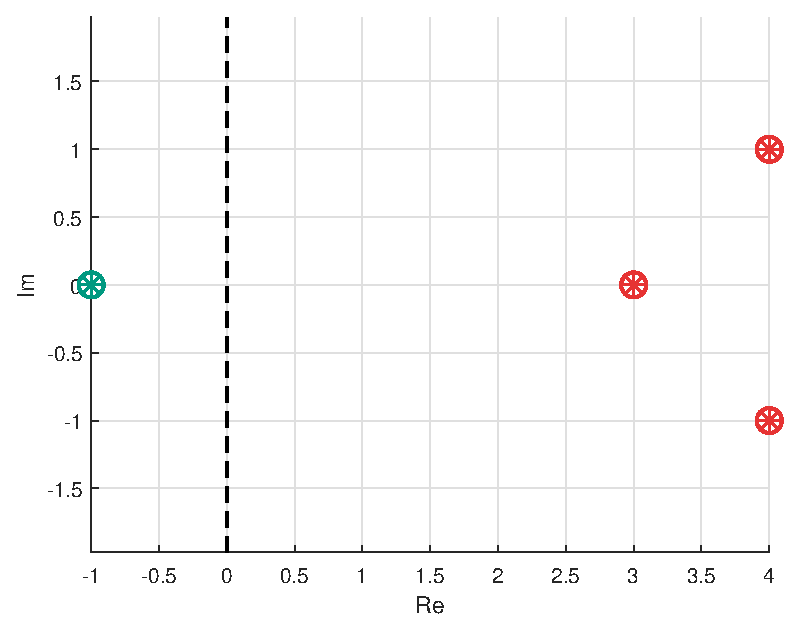
\includegraphics[width=\textwidth]{ex1/sys1/nulls_r.eps}
        \caption{Карта нулей разомкнутой системы}
        % \centerline{при $k_{\text{И}} = 0.3$, $g(t) = \sin{(0.45t)}$}
    \end{minipage}\hfill
    \begin{minipage}{0.5\textwidth}
        \centering 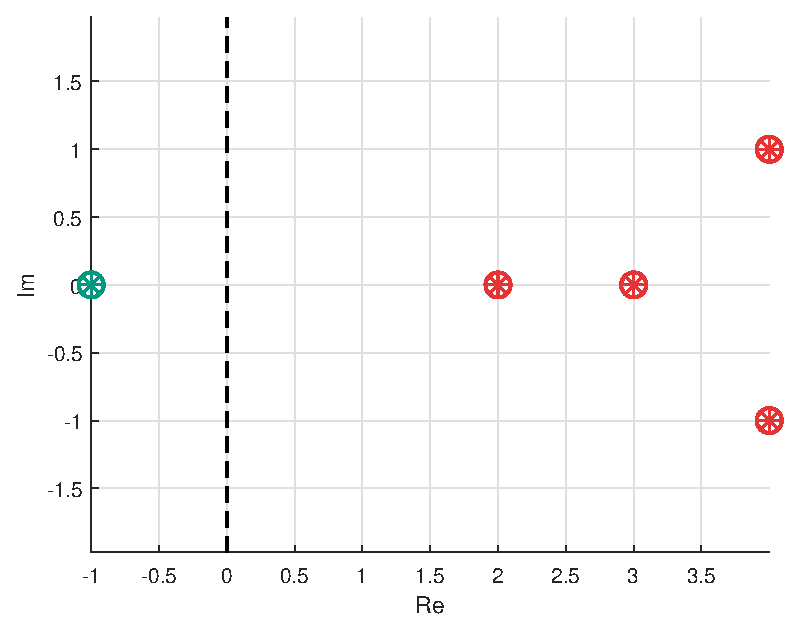
\includegraphics[width=\textwidth]{ex1/sys1/poluses_r.eps}
        \caption{Карта полюсов разомкнутой системы}
        % \centerline{при $k_{\text{И}} = 0.3$, $g(t) = \sin{(0.45t)}$}
    \end{minipage}\\[1em]
\end{figure}\noindent\


\begin{figure}[H]
    \begin{minipage}{0.5\textwidth}
        \centering 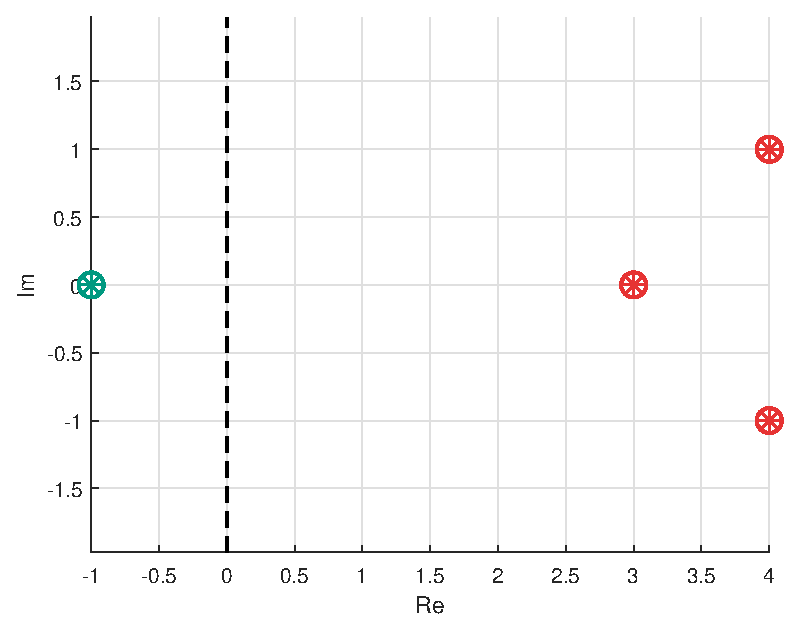
\includegraphics[width=\textwidth]{ex1/sys1/nulls.eps}
        \caption{Карта нулей замкнутой системы}
        % \centerline{при $k_{\text{И}} = 0.3$, $g(t) = \sin{(0.45t)}$}
    \end{minipage}\hfill
    \begin{minipage}{0.5\textwidth}
        \centering 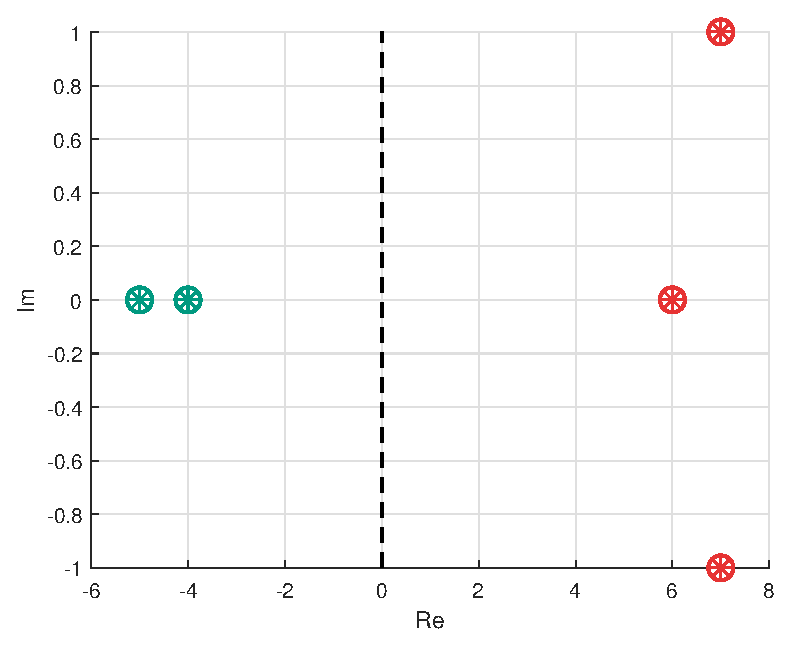
\includegraphics[width=\textwidth]{ex1/sys1/poluses.eps}
        \caption{Карта полюсов замкнутой системы}
        % \centerline{при $k_{\text{И}} = 0.3$, $g(t) = \sin{(0.45t)}$}
    \end{minipage}\\[1em]
\end{figure}\noindent\

\subsubsection{Переходные характеристики}\

\begin{figure}[H]
    \begin{minipage}{0.5\textwidth}
        \centering 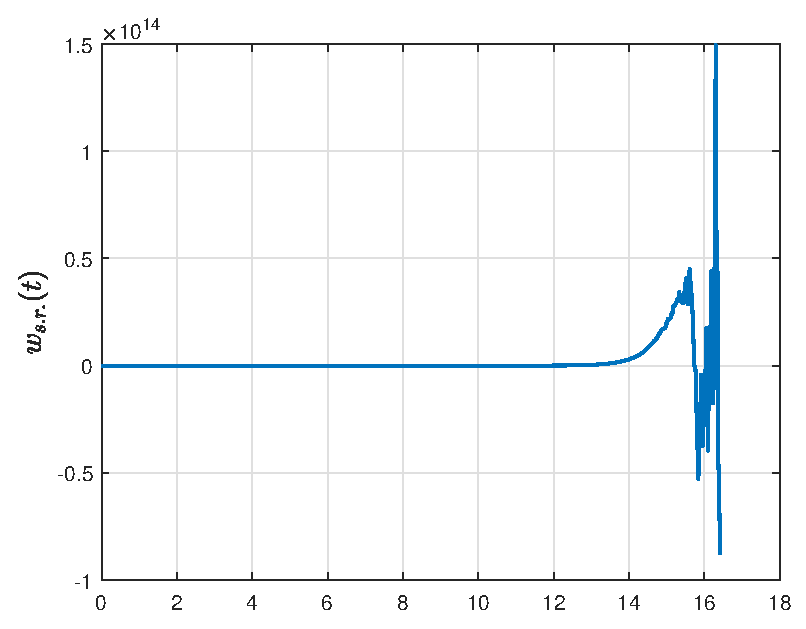
\includegraphics[width=\textwidth]{ex1/sys1/step_r.eps}
        \caption{Переходная характеристика}
        \centerline{разомкнутой системы}
    \end{minipage}\hfill
    \begin{minipage}{0.5\textwidth}
        \centering 
\includegraphics[width=\textwidth]{ex1/sys1/step.eps}
        \caption{Переходная характеристика}
        \centerline{замкнутой системы}
    \end{minipage}\\[1em]
\end{figure}\noindent\

\subsubsection{Годограф Найквиста}\

\begin{figure}[H]
    \centering
    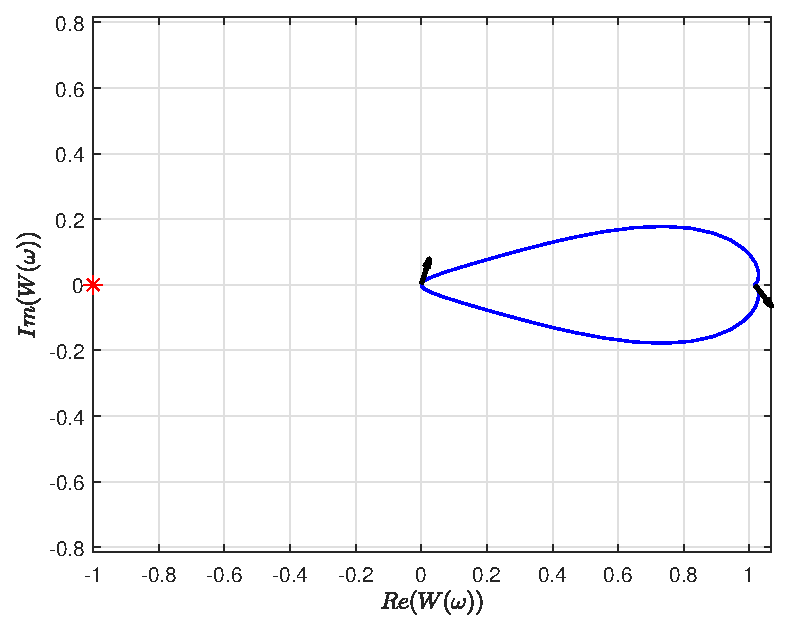
\includegraphics[width=0.55\linewidth]{ex1/sys1/niquist.eps}
    \caption{Годограф Найквиста}
\end{figure}

Годограф делает один оборот вокруг точки $(-1, 0)$ против часовой стрелки, а значит, результирующим количеством полюсов с положительной вещественной частью в замкнутой системе будет являться $4 - 1 = 3$.

\subsubsection{ЛАЧХ и ЛФЧХ разомкнутой системы}\

\begin{figure}[H]
    \centering
    
\includegraphics[width=0.50\linewidth]{ex1/sys1/fchh.eps}
    \caption{ЛФЧХ разомкнутой системы}
\end{figure}

\begin{figure}[H]
    \centering
    
\includegraphics[width=0.50\linewidth]{ex1/sys1/achh.eps}
    \caption{ЛАЧХ разомкнутой системы}
\end{figure}

График ЛАЧХ проходит через точку $L(\omega) = 0$ при частоте $\omega_1 \approx 3.5$, и после этой частоты принимает отрицательные значения. Рассмотрим требуемый по логарифмическому критерию Найквиста промежуток до $\omega_1$ по $\omega$. На отображённом промежутке график ЛФЧХ не проходит через критические отрезки, однако в пределе при $\omega \to \infty$ будет достигнут один положительный переход на критической частоте $\varphi = -\pi$, засчитываемый за $1/2$1. Тогда число неустойчивых полюсов замкнутой системы будет равняться $4-(1/2)\cdot2 = 3$ что подтверждает результат, полученный из анализа АФЧХ.

\subsection{Второй объект}\

В качестве разомкнутой системы была выбрана передаточная функция

\[
W(s) = \frac{P(s)}{(s+1)(s+2)(s+3)(s+4+j)(s+4-j)},
\]\ 

имеющая полюса $s_1 = -1, s_2 = -2, s_{3} = -3, s_{4, 5} = -4 \pm j$. Соответствующая ей передаточная функция замкнутой системы выглядит следующим образом:


\[
W_\text{З}(s) = \frac{P(s)}{P(s) + Q(s)}
\]

По заданию она должна иметь 3 неустойчивых полюса, тогда пусть её полюсами будут $s_1 = -1, s_2 = -2, s_{3} = 3, s_{4, 5} = 4 \pm j$. Тогда имеем:

\[
W_\text{З}(s) = \frac{P(s)}{P(s) + Q(s)} = \frac{P(s)}{P(s) + (s+1)(s+2)(s+3)(s+4+j)(s+4-j)} = \frac{P(s)}{(s+1)(s+2)(s-3)(s-4-j)(s-4+j)}.
\]

Приравняем знаменатели:

\[
P(s) + (s+1)(s+2)(s+3)(s+4+j)(s+4-j) = (s+1)(s+2)(s-3)(s-4-j)(s-4+j) \Leftrightarrow
\]

\[\Leftrightarrow
P(s) + s^5 +14s^4 + 76s^3 + 196s^2 + 235s + 102 = s^5 -8s^4 + 10s^3 + 50s^2 - 71s - 102 \Leftrightarrow
\]

\[\Leftrightarrow
P(s) = -22s^4 - 66s^3 - 146s^2 - 306s - 204.
\]

Тогда искомая передаточная функция:

\[
W_\text{З}(s) = \frac{-22s^4 - 66s^3 - 146s^2 - 306s - 204}{s^5 -8s^4 + 10s^3 + 50s^2 - 71s - 102}.
\]

\subsubsection{Карты нулей и полюсов}\


\begin{figure}[H]
    \begin{minipage}{0.5\textwidth}
        \centering 
\includegraphics[width=\textwidth]{ex1/sys2/nulls_r.eps}
        \caption{Карта нулей разомкнутой системы}
        % \centerline{при $k_{\text{И}} = 0.3$, $g(t) = \sin{(0.45t)}$}
    \end{minipage}\hfill
    \begin{minipage}{0.5\textwidth}
        \centering 
\includegraphics[width=\textwidth]{ex1/sys2/poluses_r.eps}
        \caption{Карта полюсов разомкнутой системы}
        % \centerline{при $k_{\text{И}} = 0.3$, $g(t) = \sin{(0.45t)}$}
    \end{minipage}\\[1em]
\end{figure}\noindent\


\begin{figure}[H]
    \begin{minipage}{0.5\textwidth}
        \centering 
\includegraphics[width=\textwidth]{ex1/sys2/nulls.eps}
        \caption{Карта нулей замкнутой системы}
        % \centerline{при $k_{\text{И}} = 0.3$, $g(t) = \sin{(0.45t)}$}
    \end{minipage}\hfill
    \begin{minipage}{0.5\textwidth}
        \centering 
\includegraphics[width=\textwidth]{ex1/sys2/poluses.eps}
        \caption{Карта полюсов замкнутой системы}
        % \centerline{при $k_{\text{И}} = 0.3$, $g(t) = \sin{(0.45t)}$}
    \end{minipage}\\[1em]
\end{figure}\noindent\

\subsubsection{Переходные характеристики}\

\begin{figure}[H]
    \begin{minipage}{0.5\textwidth}
        \centering 
\includegraphics[width=\textwidth]{ex1/sys2/step_r.eps}
        \caption{Переходная характеристика}
        \centerline{разомкнутой системы}
    \end{minipage}\hfill
    \begin{minipage}{0.5\textwidth}
        \centering 
\includegraphics[width=\textwidth]{ex1/sys2/step.eps}
        \caption{Переходная характеристика}
        \centerline{замкнутой системы}
    \end{minipage}\\[1em]
\end{figure}\noindent\

\subsubsection{Годограф Найквиста}\

\begin{figure}[H]
    \centering
    
\includegraphics[width=0.55\linewidth]{ex1/sys2/niquist_r.eps}
    \caption{Годограф Найквиста}
\end{figure}

Годограф делает три оборота вокруг точки $(-1, 0)$ по часовой стрелке, а значит, результирующим количеством полюсов с положительной вещественной частью в замкнутой системе будет являться $0 + 3 = 3$.

\subsubsection{ЛАЧХ и ЛФЧХ разомкнутой системы}\

\begin{figure}[H]
    \centering
    
\includegraphics[width=0.60\linewidth]{ex1/sys2/fchh_r.eps}
    \caption{ЛФЧХ разомкнутой системы}
\end{figure}

\begin{figure}[H]
    \centering
    
\includegraphics[width=0.60\linewidth]{ex1/sys2/achh_r.eps}
    \caption{ЛАЧХ разомкнутой системы}
\end{figure}

График ЛАЧХ уходит в отрицательную область значений при приближении к резонансной частоте (при $\omega_1 \approx 1.35$), снова выходит в положительную область примерно от $\omega_2 \approx 2.15$, затем снова пересекает прямую $L(\omega) = 0$ на частоте $\omega_3 \approx 20.46$. График ЛФЧХ начинается ($\omega \to -\infty$) на 540 градусах, это отрицательный переход, засчитываем его как $-1/2$. Далее, на $\omega \in [\omega_2, \omega_3]$ график ЛФЧХ проходит ещё одно критическое значение $L(\omega) = 180$ сверху вниз. Итоговая сумма переходов ЛФЧХ получается равной $-1.5$, после умножения на $2$ получаем $-3$, значит, тогда число неустойчивых полюсов замкнутой системы составит $0 - (-3) = 3$, что и получилось при анализе годографа Найквиста.

\subsection{Третий объект}\

У передаточной функции этого объекта должно быть 4 неустойчивых полюсов у разомкнутой системы и 0 у замкнутой. В качестве разомкнутой системы была выбрана передаточная функция

\[
W(s) = \frac{P(s)}{(s+1)(s-2)(s-3)(s-4+j)(s-4-j)},
\]\ 

имеющая полюса $s_1 = -1, s_2 = 2, s_{3} = 3, s_{4, 5} = 4 \pm j$. Соответствующая ей передаточная функция замкнутой системы выглядит следующим образом:


\[
W_\text{З}(s) = \frac{P(s)}{P(s) + Q(s)}
\]

По заданию она должна иметь 0 неустойчивых полюсов, тогда пусть её полюсами будут $s_1 = -1, s_2 = -2, s_{3} = -3, s_{4, 5} = -4 \pm j$. Тогда имеем:

\[
W_\text{З}(s) = \frac{P(s)}{P(s) + Q(s)} = \frac{P(s)}{P(s) + (s+1)(s-2)(s-3)(s-4+j)(s-4-j)} = \frac{P(s)}{(s+1)(s+2)(s+3)(s+4-j)(s+4+j)}.
\]

Приравняем знаменатели:

\[
P(s) + (s+1)(s-2)(s-3)(s-4+j)(s-4-j) = (s+1)(s+2)(s+3)(s+4-j)(s+4+j) \Leftrightarrow
\]

\[\Leftrightarrow
P(s) + s^5 -12s^4 + 50s^3 -70s^2 -31s + 102 = s^5 + 14s^4 + 76s^3 + 196s^2 + 235s + 102 \Leftrightarrow
\]

\[\Leftrightarrow
P(s) = 26s^4 + 26s^3 + 266s^2 + 266s.
\]

Тогда искомая передаточная функция:

\[
W_\text{З}(s) = \frac{26s^4 + 26s^3 + 266s^2 + 266s}{s^5 + 14s^4 + 76s^3 + 196s^2 + 235s + 102}.
\]

\subsubsection{Карты нулей и полюсов}\


\begin{figure}[H]
    \begin{minipage}{0.5\textwidth}
        \centering 
\includegraphics[width=\textwidth]{ex1/sys3/nulls_r.eps}
        \caption{Карта нулей разомкнутой системы}
        % \centerline{при $k_{\text{И}} = 0.3$, $g(t) = \sin{(0.45t)}$}
    \end{minipage}\hfill
    \begin{minipage}{0.5\textwidth}
        \centering 
\includegraphics[width=\textwidth]{ex1/sys3/poluses_r.eps}
        \caption{Карта полюсов разомкнутой системы}
        % \centerline{при $k_{\text{И}} = 0.3$, $g(t) = \sin{(0.45t)}$}
    \end{minipage}\\[1em]
\end{figure}\noindent\


\begin{figure}[H]
    \begin{minipage}{0.5\textwidth}
        \centering 
\includegraphics[width=\textwidth]{ex1/sys3/nulls.eps}
        \caption{Карта нулей замкнутой системы}
        % \centerline{при $k_{\text{И}} = 0.3$, $g(t) = \sin{(0.45t)}$}
    \end{minipage}\hfill
    \begin{minipage}{0.5\textwidth}
        \centering 
\includegraphics[width=\textwidth]{ex1/sys3/poluses.eps}
        \caption{Карта полюсов замкнутой системы}
        % \centerline{при $k_{\text{И}} = 0.3$, $g(t) = \sin{(0.45t)}$}
    \end{minipage}\\[1em]
\end{figure}\noindent\

\subsubsection{Переходные характеристики}\

\begin{figure}[H]
    \begin{minipage}{0.5\textwidth}
        \centering 
\includegraphics[width=\textwidth]{ex1/sys3/step_r.eps}
        \caption{Переходная характеристика}
        \centerline{разомкнутой системы}
    \end{minipage}\hfill
    \begin{minipage}{0.5\textwidth}
        \centering 
\includegraphics[width=\textwidth]{ex1/sys3/step.eps}
        \caption{Переходная характеристика }
        \centerline{замкнутой системы}
    \end{minipage}\\[1em]
\end{figure}\noindent\

\subsubsection{Годограф Найквиста}\

\begin{figure}[H]
    \centering
    
\includegraphics[width=0.55\linewidth]{ex1/sys3/niquist_r.eps}
    \caption{Годограф Найквиста}
\end{figure}

Годограф делает четыре оборота вокруг точки $(-1, 0)$ против часовой стрелки, а значит, результирующим количеством полюсов с положительной вещественной частью в замкнутой системе будет являться $4 - 4 = 0$.

\subsubsection{ЛАЧХ и ЛФЧХ разомкнутой системы}\

\begin{figure}[H]
    \centering
    
\includegraphics[width=0.60\linewidth]{ex1/sys3/fchh_r.eps}
    \caption{ЛФЧХ разомкнутой системы}
\end{figure}

\begin{figure}[H]
    \centering
    
\includegraphics[width=0.60\linewidth]{ex1/sys3/achh_r.eps}
    \caption{ЛАЧХ разомкнутой системы}
\end{figure}

График ЛАЧХ принимает положительные значения на двух промежутках: $[0.405, 2.430]$ и $[4.202, 24.673]$. На первом промежутке график ЛФЧХ проходит критическое значение $\varphi(\omega) = -180$ снизу вверх, и на втором прмежутке проходит это же критическое значение также снизу вверх. Сумма переходов получается равной 2, и число неустойчивых полюсов замкнутой системы вычисляется как $4 - (2\cdot 2) = 0$, результат совпал с результатом анализа годографа Найквиста.

\subsubsection{Вывод по заданию}\

Выполнив задание, я убедился в эквивалентности результатов, получаемых из исследования линейных систем классическим критерием Найквиста, и его логарифмической формулировкой. Понял, что устойчивостью замкнутых систем можно управлять при помощи изменения нулей их разомкнутых версий, и научился анализировать устойчивость замкнутых систем, зная лишь разомкнутые.

\section{Коэффициент усиления}\

В соответствии с 6 вариантом были взяты следующие передаточные функции:

\[
W_1(s) = \frac{s-2}{s^2+3s+9}, W_2(s) = \frac{10s^2+10s+3}{10s^3+s^2}
\]

К функциям добавлен коэффициент усиления:

\[
W_1(s) = k\frac{s-2}{s^2+3s+9}, W_2(s) = k\frac{10s^2+10s+3}{10s^3+s^2}
\]

\subsection{Анализ первой системы}

Начну анализ с построения годографа при $k = 1$:

\begin{figure}[H]
    \centering
    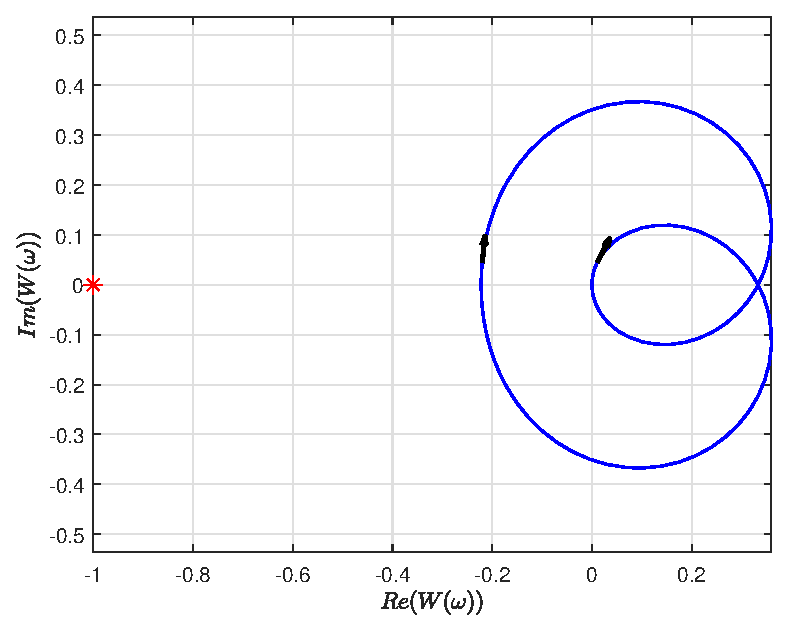
\includegraphics[width=0.60\linewidth]{ex2/sys1/niquist_r_1.eps}
    \caption{Годограф первой системы, $k = 1$}
\end{figure}

В процессе перебора значений $k$ были выбраны наиболее показательные:

\begin{figure}[H]
    \begin{minipage}{0.5\textwidth}
        \centering 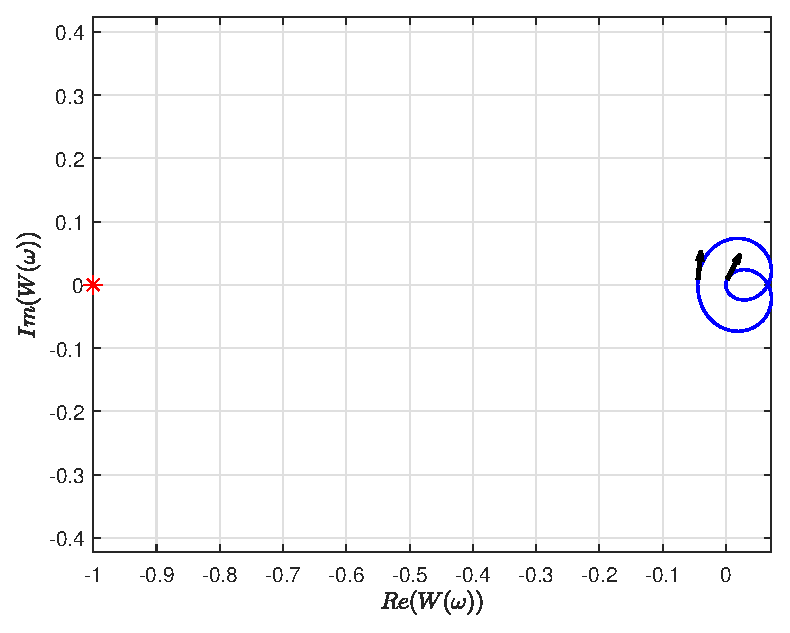
\includegraphics[width=\textwidth]{ex2/sys1/niquist_r_0.2.eps}
        \caption{Годограф первой системы, $k = 1/5$}
        % \centerline{при $k_{\text{И}} = 0.3$, $g(t) = \sin{(0.45t)}$}
    \end{minipage}\hfill
    \begin{minipage}{0.5\textwidth}
        \centering 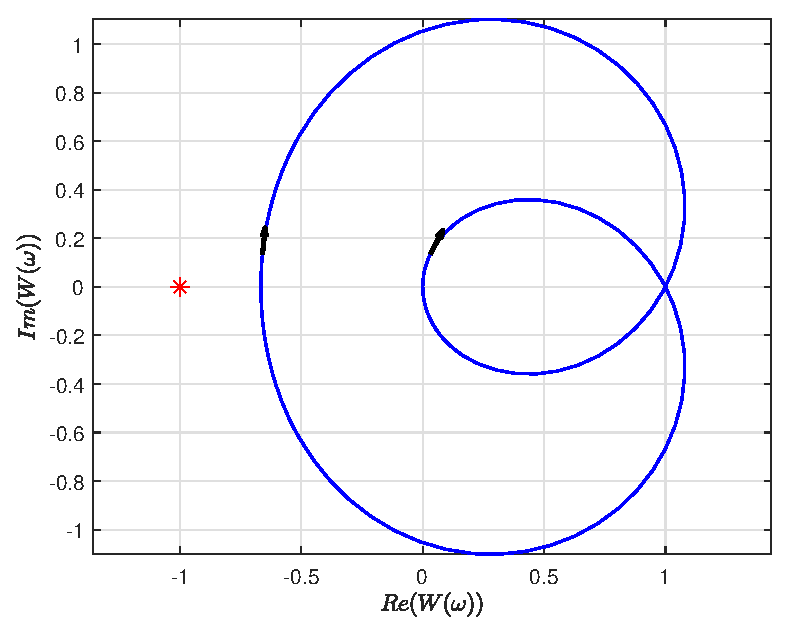
\includegraphics[width=\textwidth]{ex2/sys1/niquist_r_3.eps}
        \caption{Годограф первой системы, $k = 3$}
        % \centerline{ступенчатое воздействие}
    \end{minipage}\\[1em]
\end{figure}\noindent\

\begin{figure}[H]
    \centering
    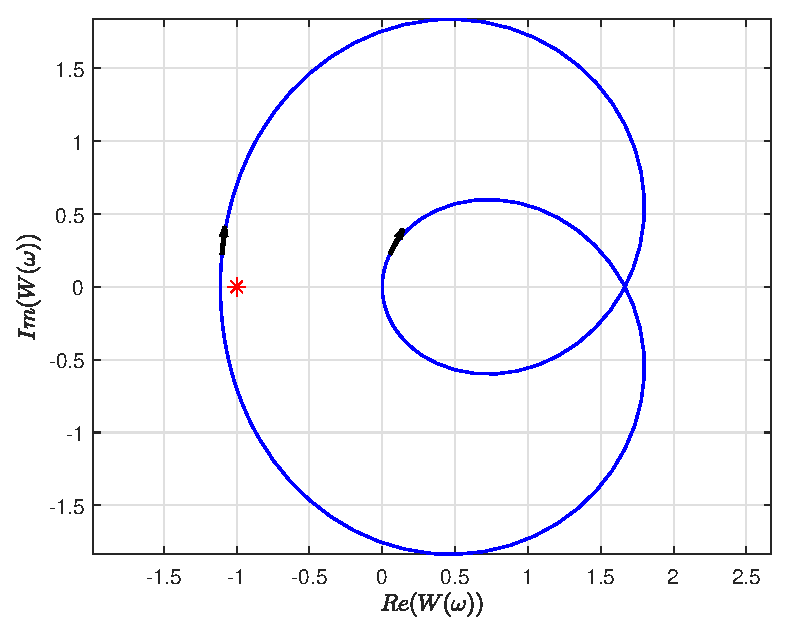
\includegraphics[width=0.60\linewidth]{ex2/sys1/niquist_r_5.eps}
    \caption{Годограф первой системы, $k = 5$}
\end{figure}

Видно, что изменение значения параметра $k$ прямо пропорционально изменению ``величины'' годографа --- амплитуда системы подвергается умножению на $k$, соответственно, меняется и длина вектора, описывающего траекторию годографа. 

Исходная разомкнутая система не имеет ни одного неустойчивого полюса, значит, если критическая точка будет охвачена хотя бы одним оборотом годографа по часовой стрелке, замкнутая система приобретёт неустойчивый характер, притом если годограф будет проходить через критическую точку, система окажется на границе устойчивости. 

Для расчета пределов значений коэффициента усиления $k$, относительно которых замкнутая система устойчива, учитывая, что полюса не сокращаются с нулями, рассмотрю знаменатель замкнутой системы:

$$1 + \frac{k(s-2)}{s^2+3s+9} = 0$$

Умножение на знаменатель:

$$(s^2+3s+9) + k(s-2) = 0$$

Соберем коэффициенты при степенях $s$:

$$s^2 + (3+k)s + (9-2k) = 0$$

По следствию из критерия Гурвица можно заключить, что замкнутая система устойчива при выполнении условий:

\[
\begin{cases}
    3+k > 0, \\
    9-2k > 0.
\end{cases} \Leftrightarrow 
\begin{cases}
    k > -3, \\
    k < 4.5.
\end{cases}
\]

При $k > 4.5$ система окажется неустойчива.

Переходные характеристики для каждой из определённых областей:

\begin{figure}[H]
    \begin{minipage}{0.5\textwidth}
        \centering 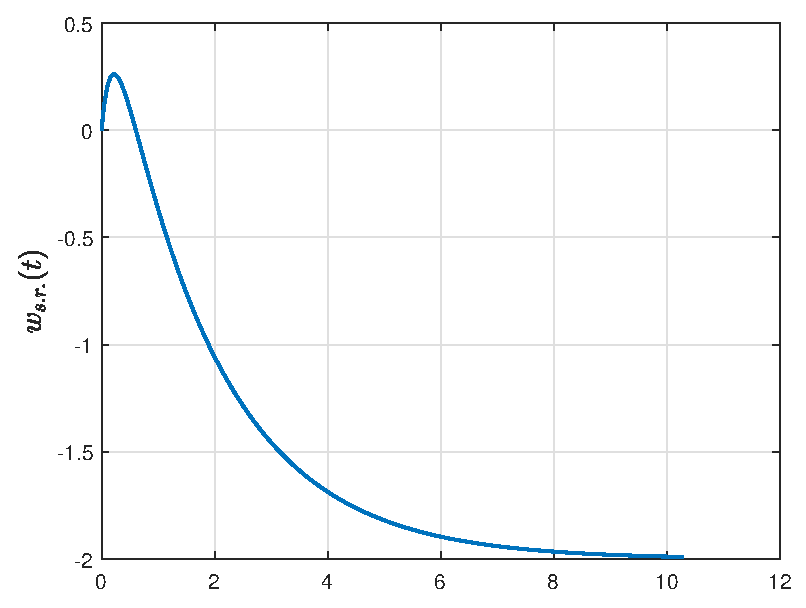
\includegraphics[width=\textwidth]{ex2/sys1/step_3.eps}
        \caption{Переходная характеристика замкнутой}
        \centerline{системы при $k = 3$}
    \end{minipage}\hfill
    \begin{minipage}{0.5\textwidth}
        \centering 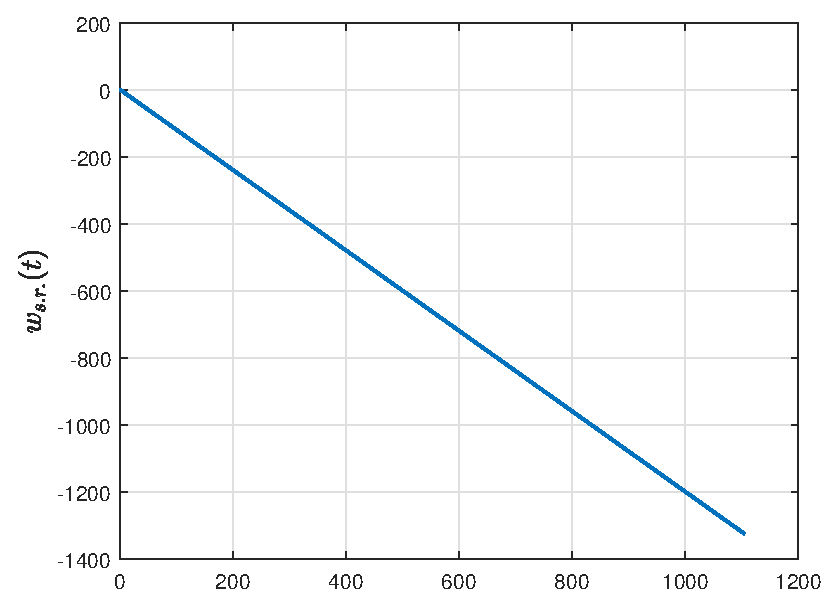
\includegraphics[width=\textwidth]{ex2/sys1/step_4.5.eps}
        \caption{Переходная характеристика замкнутой}
        \centerline{системы при $k = 4.5$}
    \end{minipage}\\[1em]
\end{figure}\noindent\


\begin{figure}[H]
    \centering
    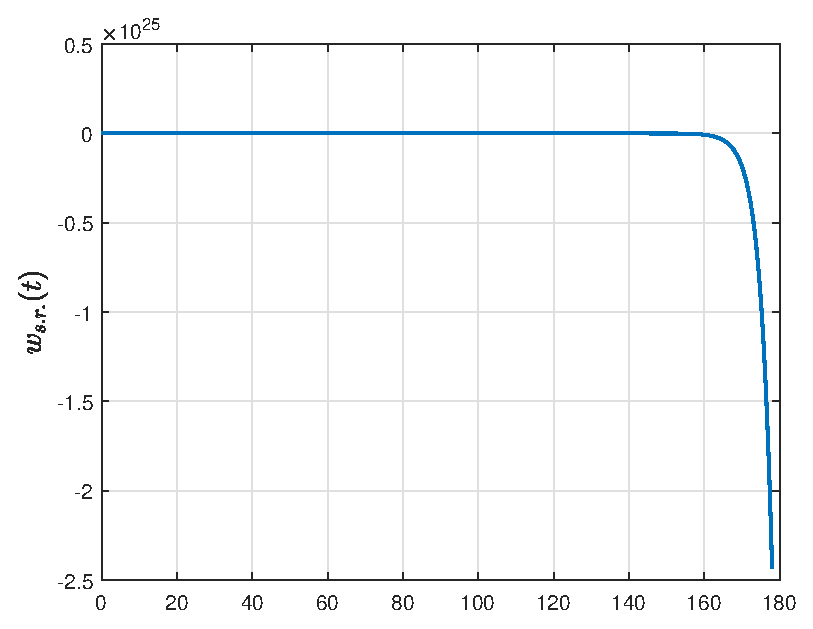
\includegraphics[width=0.60\linewidth]{ex2/sys1/step_6.eps}
        \caption{Переходная характеристика замкнутой}
        \centerline{системы при $k = 6$}
\end{figure}

\subsection{Анализ второй системы}

Передаточная функция второй системы для моего варианта:

\[
W_2(s) = k\frac{10s^2+10s+3}{10s^3+s^2}.
\]

Начну анализ с построения годографа при $k = 1$:

\begin{figure}[H]
    \centering
    
\includegraphics[width=0.60\linewidth]{ex2/sys2/niquist_r_1.eps}
    \caption{Годограф второй системы, $k = 1$}
\end{figure}

В процессе перебора значений $k$ были выбраны наиболее показательные:

\begin{figure}[H]
    \begin{minipage}{0.5\textwidth}
        \centering 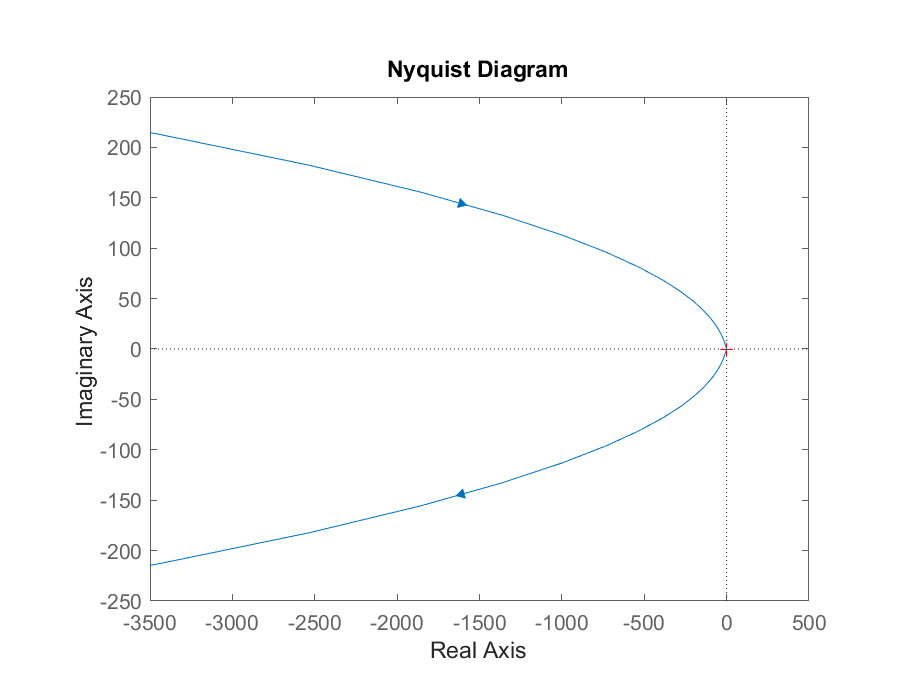
\includegraphics[width=\textwidth]{ex2/sys2/niquist_r_0.1.eps}
        \caption{Годограф второй системы, $k = 0.1$}
        % \centerline{при $k_{\text{И}} = 0.3$, $g(t) = \sin{(0.45t)}$}
    \end{minipage}\hfill
    \begin{minipage}{0.5\textwidth}
        \centering 
\includegraphics[width=\textwidth]{ex2/sys2/niquist_r_0.2.eps}
        \caption{Годограф второй системы, $k = 0.2$}
        % \centerline{ступенчатое воздействие}
    \end{minipage}\\[1em]
\end{figure}\noindent\

\begin{figure}[H]
    \centering
    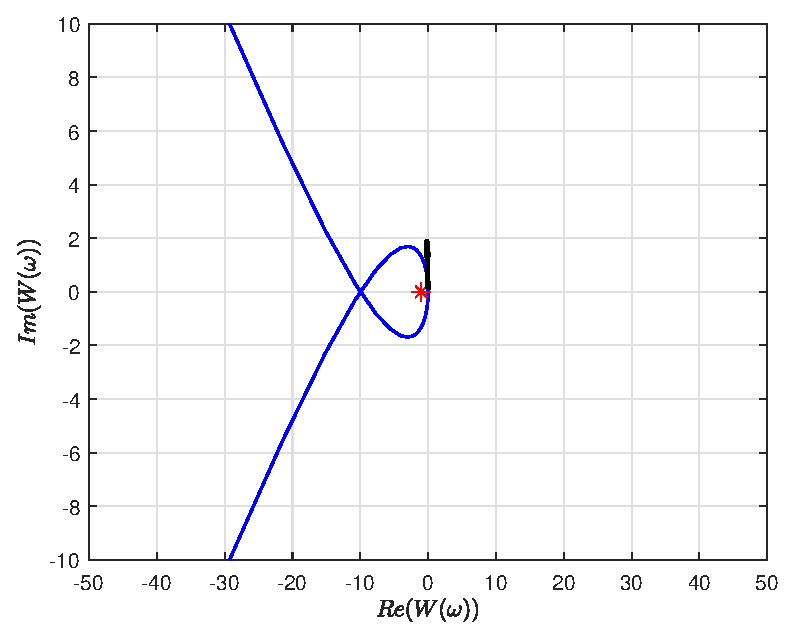
\includegraphics[width=0.60\linewidth]{ex2/sys2/niquist_r_2.eps}
    \caption{Годограф второй системы, $k = 2$}
\end{figure}

Для расчета пределов значений коэффициента усиления $k$, относительно которых замкнутая система устойчива, учитывая, что полюса не сокращаются с нулями, рассмотрю знаменатель замкнутой системы:

$$1 + k \frac{10s^2+10s+3}{10s^3+s^2} = 0$$

Умножаем на знаменатель $10s^3+s^2$:

$$(10s^3+s^2) + k(10s^2+10s+3) = 0$$

Соберем коэффициенты при степенях $s$:

\[10s^3 + (1 + 10k)s^2 + (10k)s + (3k) = 0 \Leftrightarrow s^3 + \frac{1 + 10k}{10}s^2 + ks + 0.3k = 0\]

По следствию из критерия Гурвица для системы третьего порядка можно заключить, что замкнутая система асимптотически устойчива при выполнении условий:

\[
\begin{cases}
    \frac{1 + 10k}{10} > 0, \\
    k > 0, \\
    \frac{(1 + 10k)k}{10} > 0.3k.
\end{cases} \Leftrightarrow 
\begin{cases}
    1 + 10k > 0, \\
    k > 0, \\
    (1 + 10k)k > 3k.
\end{cases} \Leftrightarrow 
\begin{cases}
    k > -0.1, \\
    k > 0, \\
    10k^2 - 2k > 0.
\end{cases} \Leftrightarrow k > 0.2.
\]

При $k < 0.2$ система окажется неустойчива.

При $k = 1$ разомкнутая система не является асимптотически устойчивой, значит, реального действующего запаса устойчивости нет. Однако никто не мешает его найти, пусть он и будет отрицательный. Для этого воспользуюсь графиками ФЧХ и АЧХ:

\begin{figure}[H]
    \centering
    
\includegraphics[width=0.50\linewidth]{ex2/sys2/achh_r_1.eps}
    \caption{АЧХ второй системы, $k = 1$}
\end{figure}

\begin{figure}[H]
    \centering
    
\includegraphics[width=0.50\linewidth]{ex2/sys2/fchh_r_1.eps}
    \caption{ФЧХ второй системы, $k = 1$}
\end{figure}

$\varphi(\omega)$ принимает значение $-180^{\circ}$ при $\omega_{\text{кр}} \approx 0.446$, на этой частоте $A(\omega_{\text{кр}}) \approx 5.03$. $\omega_\text{кр} < \omega_\text{ср}$, поэтому запас по амплитуде действительно отрицательный, реальным запасом не является. 

Переходные характеристики для каждой из определённых областей:

\begin{figure}[H]
    \begin{minipage}{0.5\textwidth}
        \centering 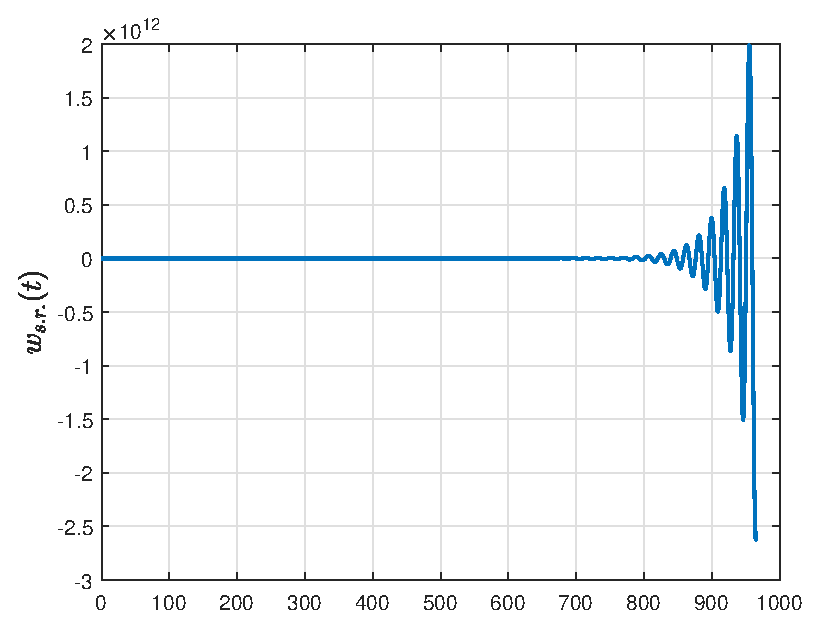
\includegraphics[width=\textwidth]{ex2/sys2/step_0.1.eps}
        \caption{Переходная характеристика замкнутой}
        \centerline{системы при $k = 0.1$}
    \end{minipage}\hfill
    \begin{minipage}{0.5\textwidth}
        \centering 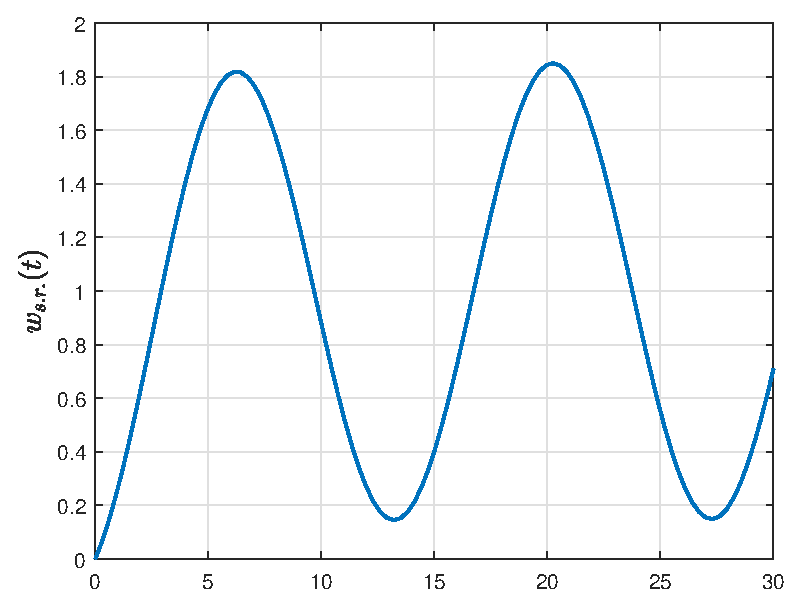
\includegraphics[width=\textwidth]{ex2/sys2/step_0.2.eps}
        \caption{Переходная характеристика замкнутой}
        \centerline{системы при $k = 0.2$}
    \end{minipage}\\[1em]
\end{figure}\noindent\


\begin{figure}[H]
    \centering
    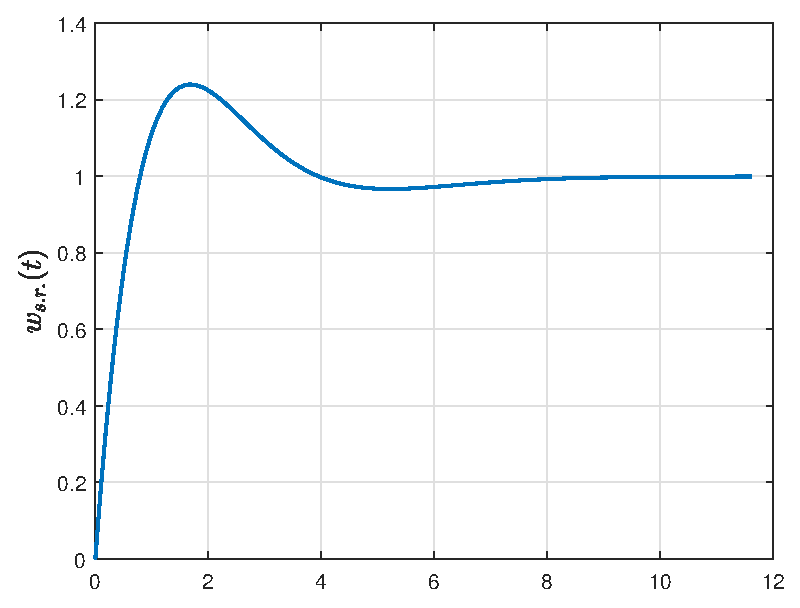
\includegraphics[width=0.60\linewidth]{ex2/sys2/step_2.eps}
        \caption{Переходная характеристика замкнутой}
        \centerline{системы при $k = 2$}
\end{figure}

\subsection{Выводы по заданию}\

Выполнив задание, я приобрёл навык подбора нужного значения коэффициента усиления, узнал, что с его помощью можно масштабировать годограф Найквиста, меняя тип устойчивости системы.

\section{Запаздывание}

В задании рассматриваются следующие системы с запаздыванием:

\[
W_3(s) = \frac{9s+3}{s^2+3s+5}e^{-s\tau}, W_4(s) = \frac{10s^2-6s+11}{10s^3-s^2+38s+20}e^{-s\tau}
\]

\subsection{Первая система}

Для первой системы с коэффициентами запаздывания $\tau=0$ и $\tau=0.5$ были построены АФЧХ:

\begin{figure}[H]
    \begin{minipage}{0.5\textwidth}
        \centering 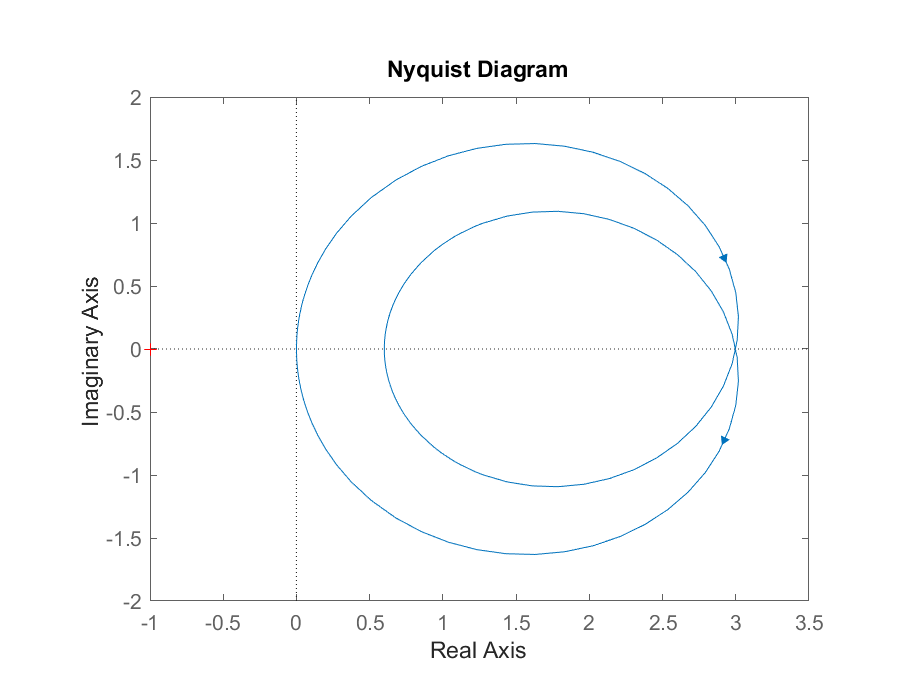
\includegraphics[width=\textwidth]{ex3/sys1/T0.eps}
        \caption{Годограф Найквиста первой}
        \centerline{системы при $\tau = 0$}
    \end{minipage}\hfill
    \begin{minipage}{0.5\textwidth}
        \centering 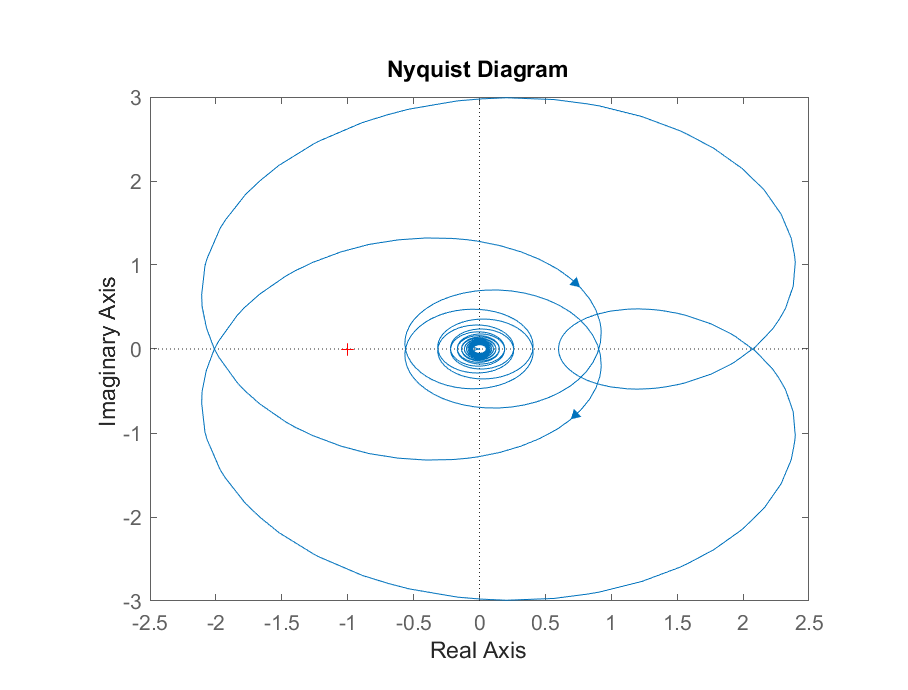
\includegraphics[width=\textwidth]{ex3/sys1/T0.5.eps}
        \caption{Годограф Найквиста первой}
        \centerline{системы при $\tau = 0.5$}
    \end{minipage}\\[1em]
\end{figure}\noindent\

Для изучения влияния параметра $\tau$ на вид годографа система была промоделирована с разными значениями этого параметра:

\begin{figure}[H]
    \begin{minipage}{0.5\textwidth}
        \centering 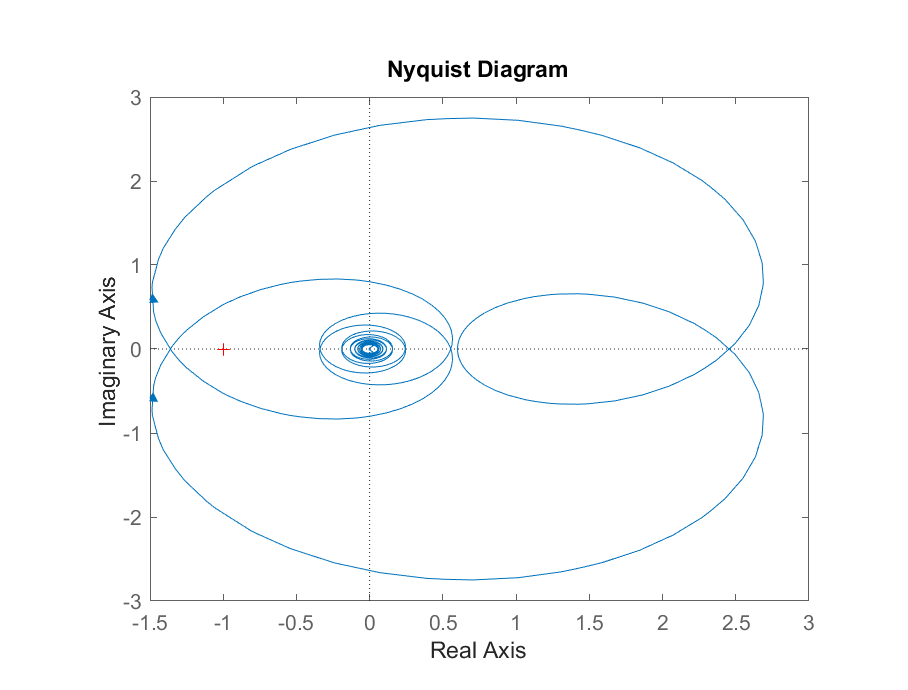
\includegraphics[width=\textwidth]{ex3/sys1/T0.3.eps}
        \caption{Годограф Найквиста первой}
        \centerline{системы при $\tau = 0.3$}
    \end{minipage}\hfill
    \begin{minipage}{0.5\textwidth}
        \centering 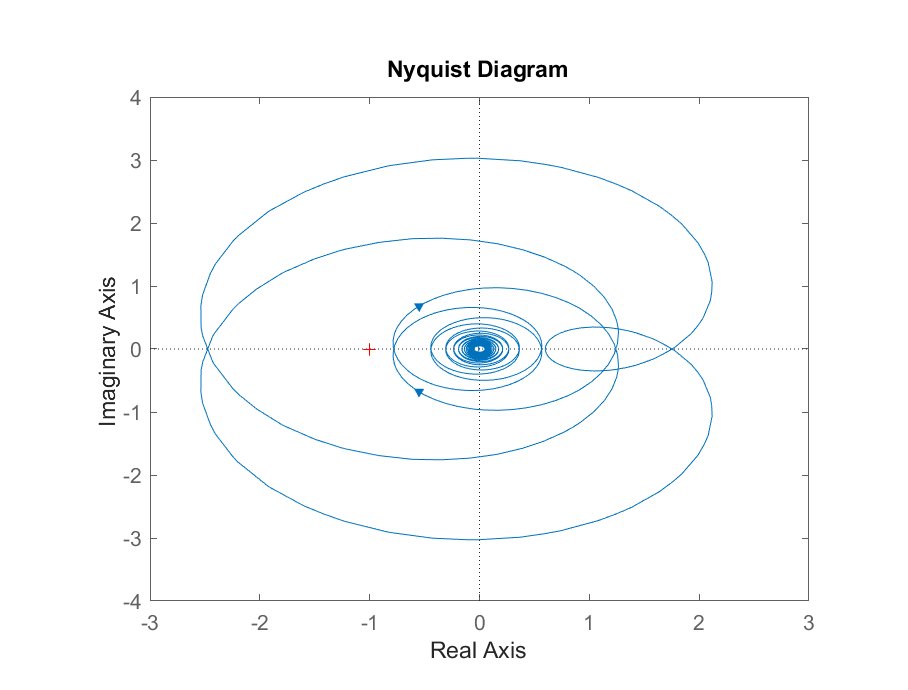
\includegraphics[width=\textwidth]{ex3/sys1/T0.7.eps}
        \caption{Годограф Найквиста первой}
        \centerline{системы при $\tau = 0.7$}
    \end{minipage}\\[1em]
\end{figure}\noindent\

\begin{figure}[H]
    \centering 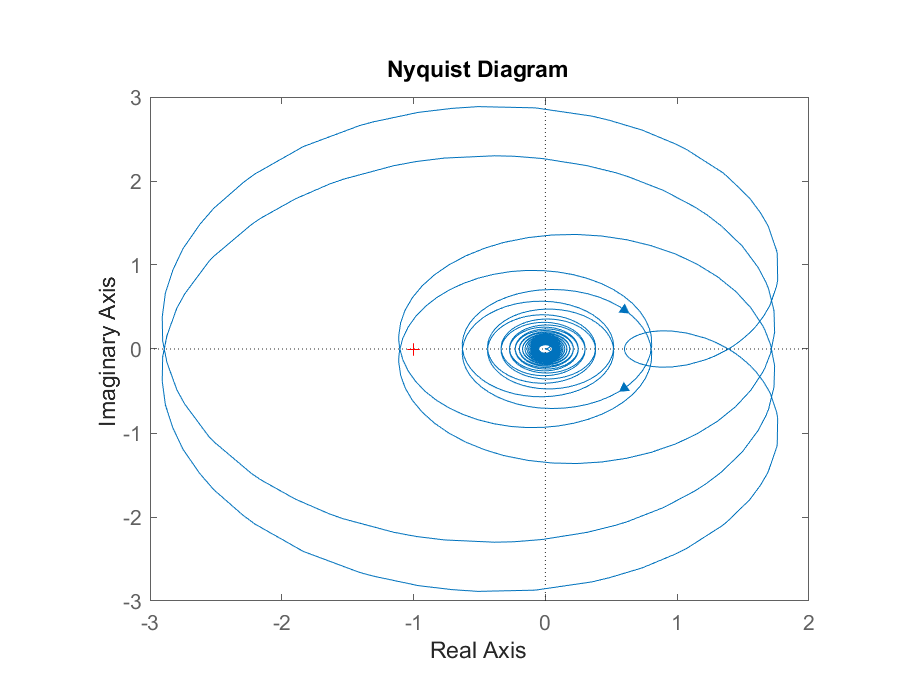
\includegraphics[width=0.65\textwidth]{ex3/sys1/T1.eps}
    \caption{Годограф Найквиста первой}
    \centerline{системы при $\tau = 1$}
\end{figure}

Заметно, что с увеличением значения параметра $\tau$ на графике вокруг начала координат становится больше линий, больше вращений. 

С введением запаздывания в системе появляется сдвиг фазы, при этом амплитуда не меняется. Тогда, для поиска критического запаздывания, при котором система перестанет быть устойчивой, нужно на годографе Найквиста, построенном без запаздывания, найти частоту, при которой амплитуда равняется 1 (критическая точка на расстоянии 1 от начала координат), найти фазу, наблюдаемую на этой частоте. 

\begin{figure}[H]
    \centering 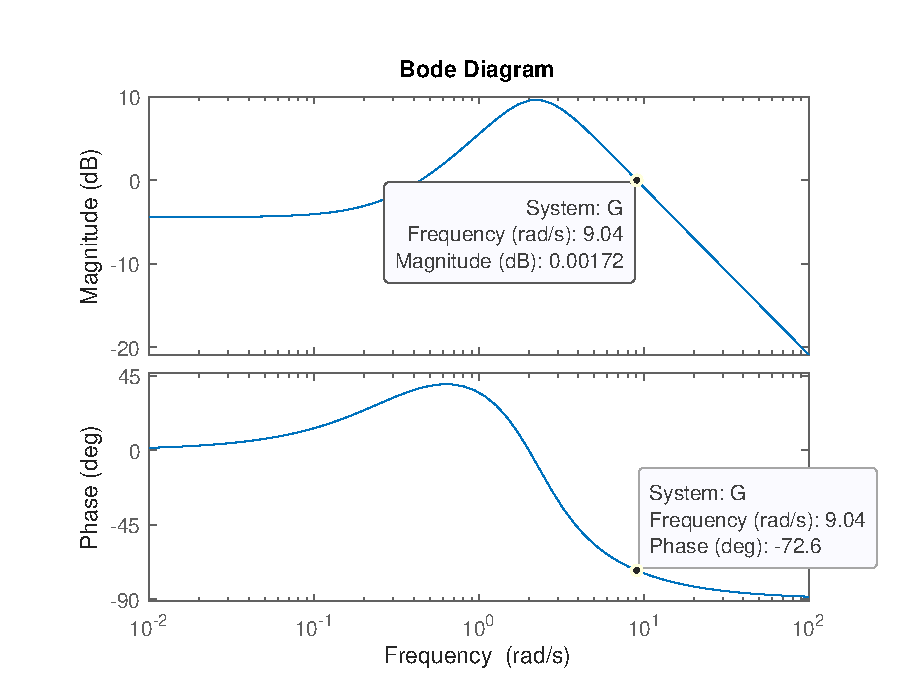
\includegraphics[width=0.60\textwidth]{ex3/sys1/A1.eps}
    \caption{Графики ЛАЧХ и ЛФЧХ первой}
    \centerline{системы при $\tau = 0$}
\end{figure}

Из рисунка видно, что на нужной частоте $\omega_{\text{ср}} \approx 9.04$ фаза равняется примерно $-72.6$ градусам.В радианах это $\frac{-72.6\pi}{180}\approx-1.2671$. Тогда запас по фазе как отклонение от критического значения фазы $\varphi = \pi$ составляет $\varphi_\text{з} = \pi-1.2671 \approx 1.8745$ радиан.

Учитывая это, можно найти критическое запаздывание по формуле, предложенной на практическом занятии, выведенной из свойства фазо-частотной характеристики системы с запаздыванием:

\[
\tau_{max} = \frac{\varphi_\text{з}}{\omega_{\text{ср}}} = \frac{1.8745}{9.04} \approx 0.2074.
\]

Были промоделированы переходные характеристики замкнутой системы при различных значениях запаздывания:

\begin{figure}[H]
    \begin{minipage}{0.5\textwidth}
        \centering 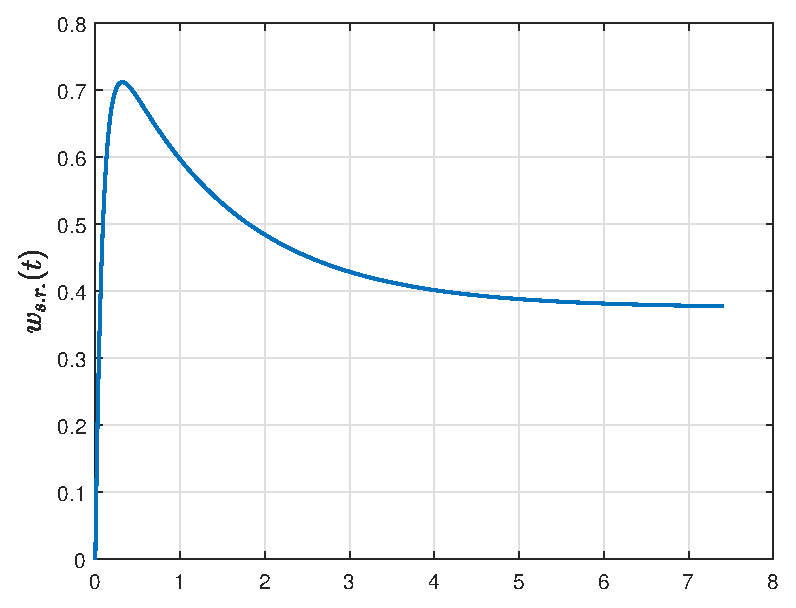
\includegraphics[width=\textwidth]{ex3/sys1/step_0.eps}
        \caption{Переходная характеристика первой}
        \centerline{системы при $\tau = 0$}
    \end{minipage}\hfill
    \begin{minipage}{0.5\textwidth}
        \centering 
\includegraphics[width=\textwidth]{ex3/sys1/step_0.1.eps}
        \caption{Переходная характеристика первой}
        \centerline{системы при $\tau = 0.1$}
    \end{minipage}\\[1em]
\end{figure}\noindent\

\begin{figure}[H]
    \begin{minipage}{0.5\textwidth}
        \centering 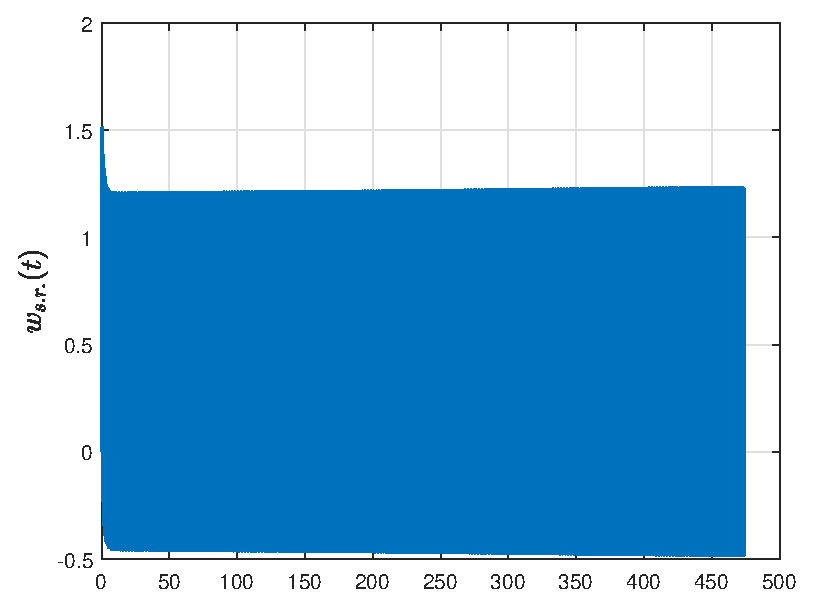
\includegraphics[width=\textwidth]{ex3/sys1/step_0.20717.eps}
        \caption{Переходная характеристика первой}
        \centerline{системы при $\tau \approx \tau_{max}$}
    \end{minipage}\hfill
    \begin{minipage}{0.5\textwidth}
        \centering 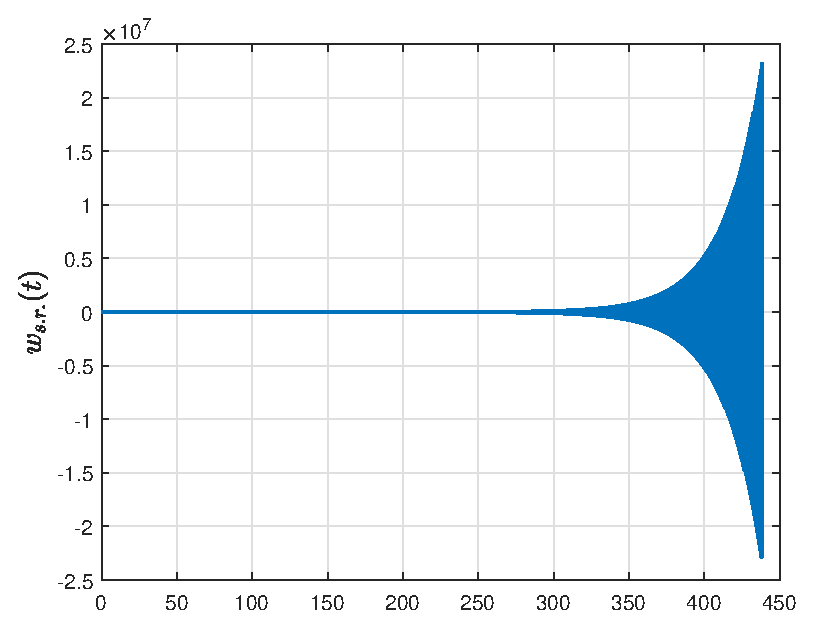
\includegraphics[width=\textwidth]{ex3/sys1/step_0.21.eps}
        \caption{Переходная характеристика первой}
        \centerline{системы при $\tau = 0.21$}
    \end{minipage}\\[1em]
\end{figure}\noindent\

\subsection{Вторая система}

Для второй системы

\[
W_4(s) = \frac{10s^2-6s+11}{10s^3-s^2+38s+20}e^{-s\tau}
\]

с коэффициентами запаздывания $\tau=0$ и $\tau=0.5$ были построены АФЧХ:

\begin{figure}[H]
    \begin{minipage}{0.5\textwidth}
        \centering 
\includegraphics[width=\textwidth]{ex3/sys2/T0.eps}
        \caption{Годограф Найквиста второй}
        \centerline{системы при $\tau = 0$}
    \end{minipage}\hfill
    \begin{minipage}{0.5\textwidth}
        \centering 
\includegraphics[width=\textwidth]{ex3/sys2/T0.5.eps}
        \caption{Годограф Найквиста вторй}
        \centerline{системы при $\tau = 0.5$}
    \end{minipage}\\[1em]
\end{figure}\noindent\

Для изучения влияния параметра $\tau$ на вид годографа система была промоделирована с разными значениями этого параметра:

\begin{figure}[H]
    \begin{minipage}{0.5\textwidth}
        \centering 
\includegraphics[width=\textwidth]{ex3/sys2/T0.3.eps}
        \caption{Годограф Найквиста второй}
        \centerline{системы при $\tau = 0.3$}
    \end{minipage}\hfill
    \begin{minipage}{0.5\textwidth}
        \centering 
\includegraphics[width=\textwidth]{ex3/sys2/T0.7.eps}
        \caption{Годограф Найквиста второй}
        \centerline{системы при $\tau = 0.7$}
    \end{minipage}\\[1em]
\end{figure}\noindent\

\begin{figure}[H]
    \centering 
\includegraphics[width=0.65\textwidth]{ex3/sys2/T1.eps}
    \caption{Годограф Найквиста второй системы при $\tau = 1$}
    % \centerline{системы при $\tau = 1$}
\end{figure}

В случае с этой системой полезно посмотреть на карту полюсов разомкнутой системы:

\begin{figure}[H]
    \centering 
\includegraphics[width=0.6\textwidth]{ex3/sys2/poluses.eps}
    \caption{Карта полюсов разомкнутой системы при отсутствии запаздывания}
    % \centerline{системы при $\tau = 1$}
\end{figure}

Видно, что система имеет два неустойчивых полюса.

По графикам годографа Найквиста заметно, что с увеличением значения параметра $\tau$ на графике вокруг начала координат становится больше вращений. При отсутствии запаздывания годограф не охватывает критическую точку, затем, при некотором значении запаздывания начинает охватывать её дважды, компенсируя неустойчивые полюса разомкнутой системы и делая замкнутую устойчивой, далее с некоторого значения величины запаздывания годограф перестаёт охватывать критическую точку, и замкнутая система становится неустойчива.

Найду критическое запаздывание для этой системы. Для этого проанализирую графики ЛАЧХ и ЛФЧХ разомкнутой системы с коэффициентом запаздывания $\tau=0$.

\begin{figure}[H]
    \centering 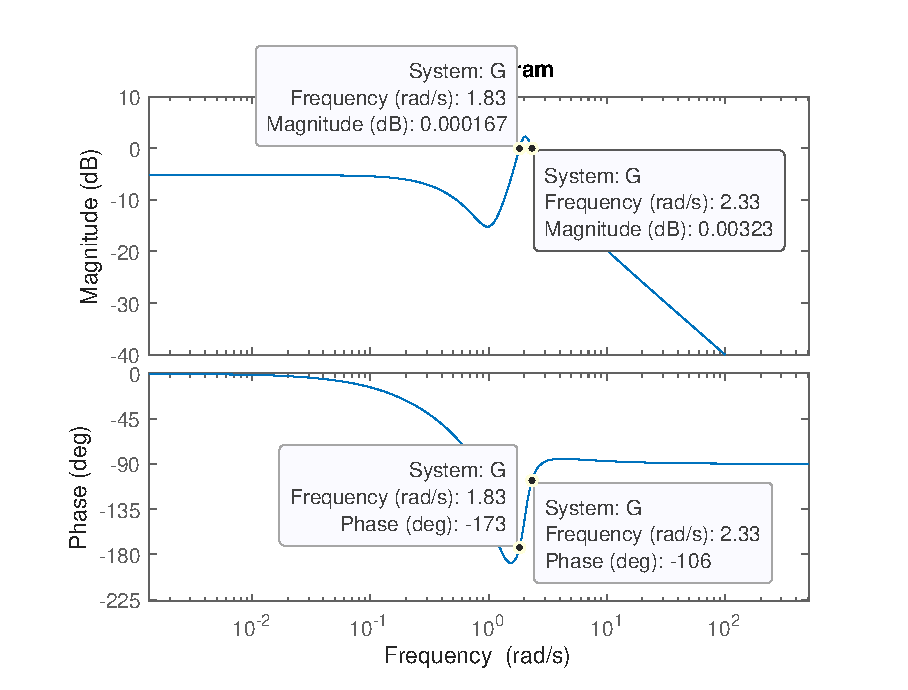
\includegraphics[width=0.65\textwidth]{ex3/sys2/A1_1.eps}
    \caption{Графики ЛАЧХ и ЛФЧХ второй системы при $\tau = 0$}
    % \centerline{}
\end{figure}

Из рисунка видно, что на частоте $\omega_{\text{ср}} \approx 2.33$ фаза равняется примерно $-106.65$ градусам. В радианах это $\frac{-106.65\pi}{180}\approx-1.8614$. Тогда запас по фазе как отклонение от критического значения фазы $\varphi = \pi$ составляет $\varphi_\text{з} = \pi-1.8614 \approx 1.2802$ радиан. Реального запаса по фазе не будет, так как система неустойчива, но использовать это значение в расчётах это не мешает.

Учитывая это, можно найти критическое запаздывание по формуле, предложенной на практическом занятии, выведенной из свойства фазо-частотной характеристики системы с запаздыванием:

\[
\tau_{max} = \frac{\varphi_\text{з}}{\omega_{\text{ср}}} = \frac{1.2802}{2.33} \approx 0.549.
\]

Найдено значение, при котором система перестаёт быть устойчивой. Также из анализа годографов для различных $\tau$ и карты полюсов разомкнутой системы известно, что в отсутствие запаздывания замкнутая система также не устойчива, и можно попробовать найти то значение устойчивости, при котором система из неустойчивой становится устойчивой. Для этого, снова посмотрев на Графики ЛАЧХ и ЛФЧХ, можно проанализировать ещё одно значение частоты среза $\omega_{\text{ср1}} \approx 1.83$. $\varphi(\omega_{\text{ср1}}) \approx -174.39$. В радианах это $\frac{-174.39\pi}{180}\approx-3.0437$. Тогда запас по фазе как отклонение от критического значения фазы $\varphi = \pi$ составляет $\varphi_\text{з1} = \pi-3.0437 \approx 0.0979$ радиан.

Учитывая это, можно найти второе критическое запаздывание:

\[
\tau_{min} = \frac{\varphi_\text{з1}}{\omega_{\text{ср1}}} = \frac{0.0979}{1.83} \approx 0.0535.
\]

Резюмируя результаты подсчётов критических значений запаздывания, можно выделить следующие промежутки:
\begin{itemize}
    \item $\tau<0.0979$ --- замкнутая система неустойчива;
    \item $\tau>0.0979$ и $\tau<0.549$ --- замкнутая система асимптотически устойчива;
    \item $\tau>0.549$ --- замкнутая система не устойчива.
\end{itemize}

Замкнутая система была промоделирована, ниже приведены полученные переходные характеристики при различных значениях запаздывания.

\begin{figure}[H]
    \begin{minipage}{0.5\textwidth}
        \centering 
\includegraphics[width=\textwidth]{ex3/sys2/step_0.eps}
        \caption{Переходная характеристика второй}
        \centerline{системы при $\tau = 0$}
    \end{minipage}\hfill
    \begin{minipage}{0.5\textwidth}
        \centering 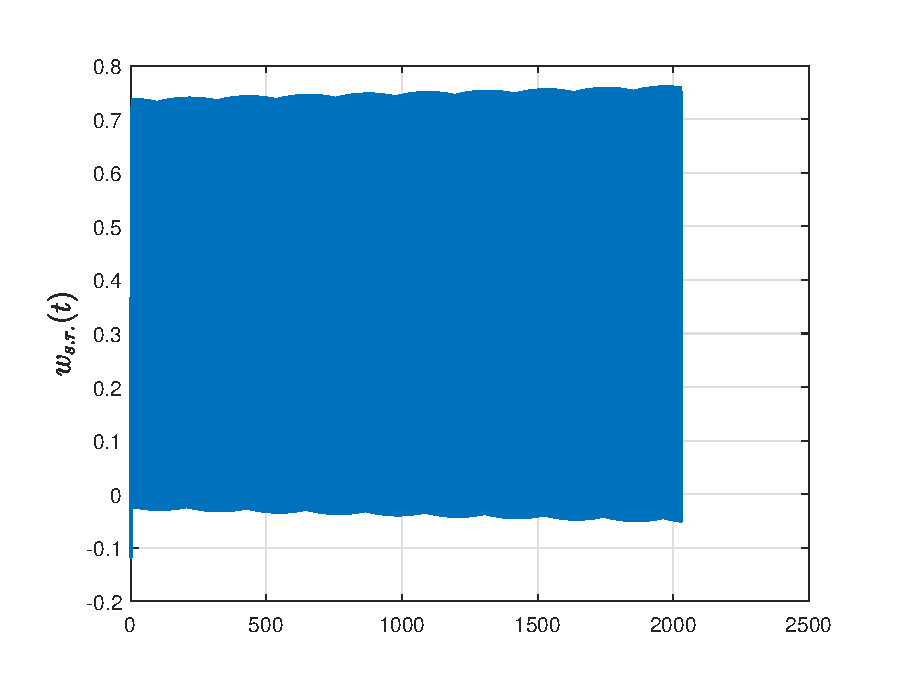
\includegraphics[width=\textwidth]{ex3/sys2/step_min.eps}
        \caption{Переходная характеристика второй}
        \centerline{системы при $\tau \approx \tau_{min}$}
    \end{minipage}\\[1em]
\end{figure}\noindent\

\begin{figure}[H]
    \begin{minipage}{0.5\textwidth}
        \centering 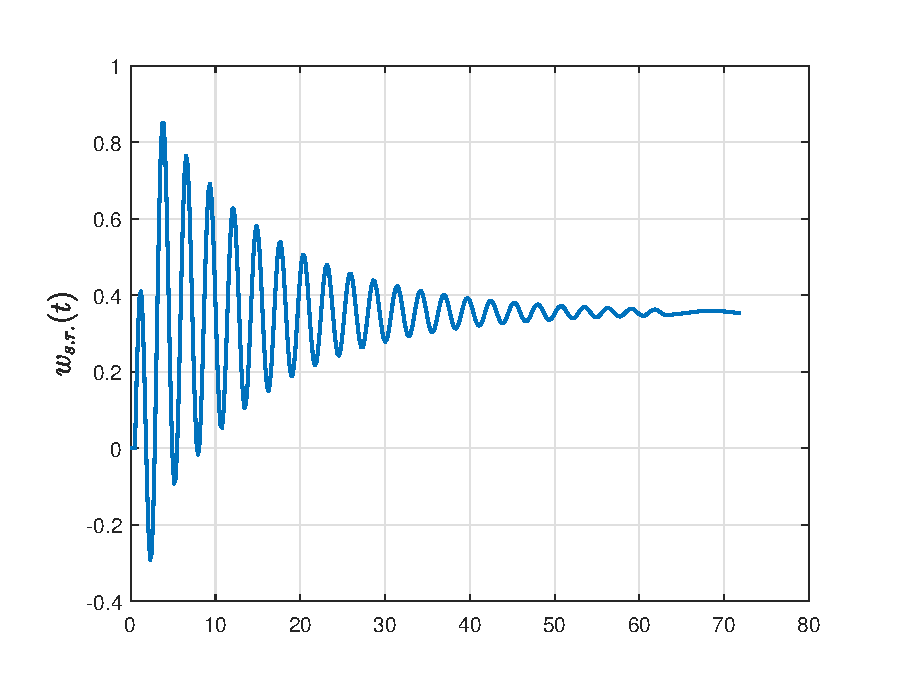
\includegraphics[width=\textwidth]{ex3/sys2/step_0.5.eps}
        \caption{Переходная характеристика второй}
        \centerline{системы при $\tau = 0.5$}
    \end{minipage}\hfill
    \begin{minipage}{0.5\textwidth}
        \centering 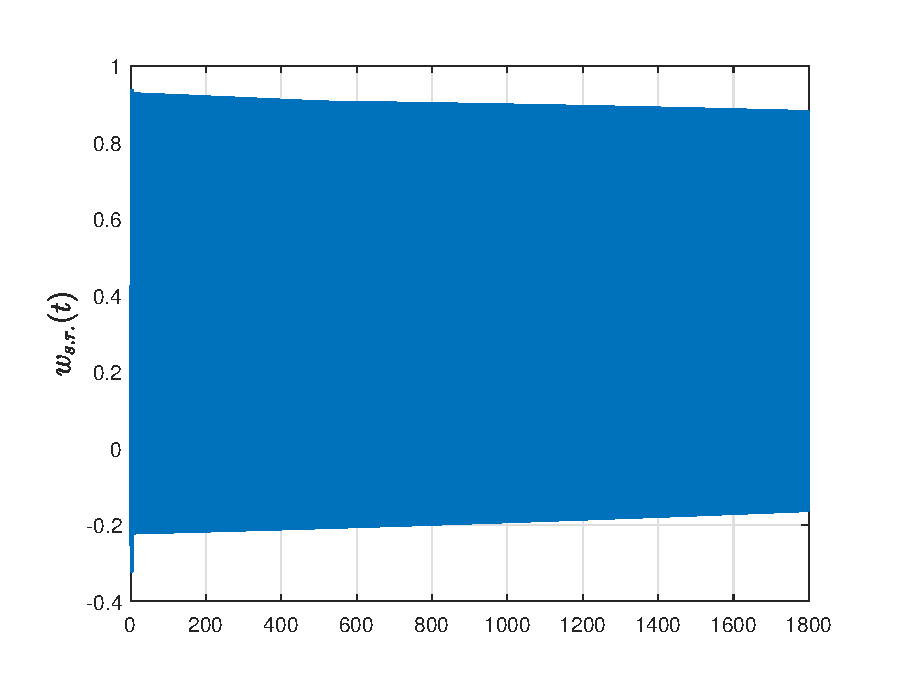
\includegraphics[width=\textwidth]{ex3/sys2/step_0.5554.eps}
        \caption{Переходная характеристика второй}
        \centerline{системы при $\tau \approx \tau_{max}$}
    \end{minipage}\\[1em]
\end{figure}\noindent\

\begin{figure}[H]
    \centering 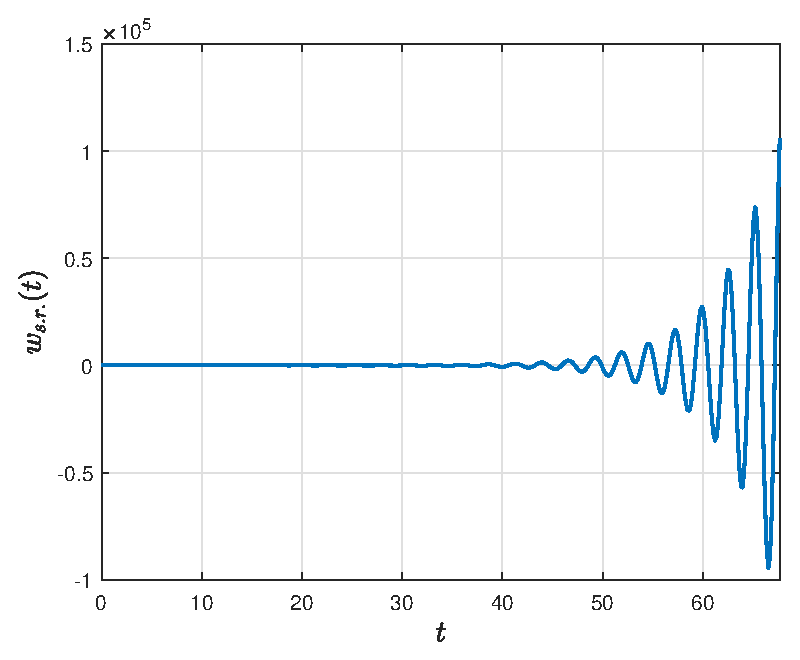
\includegraphics[width=0.65\textwidth]{ex3/sys2/step_0.7.eps}
    \caption{Переходная характеристика второй системы при $\tau = 0.7$}
    % \centerline{}
\end{figure}

\subsection{Вывод по заданию}\

Выполнив задание, я ознакомился с запаздыванием, его влиянием на годограф Найквиста и на устойчивость замкнутой системы.

\section{Вывод по работе}\

В процессе выполнения работы я ознакомился с системами с запаздыванием, формулировками и применением критерия Найквиста, а также с влиянием коэффициента усиления на устойчивость линейных систем.

\section{Приложение А. Код для выполнения заданий}

\subsection*{Листинг 1. Код для выполнения задания 1}

\begin{lstlisting}[caption={Код для построения графиков для задания 1}, language=matlab]
clear all;
close all;
raz = '_r'; % разомкнутую ли систему строим? (для сохранения графиков)
[~, scriptName] = fileparts(mfilename('fullpath'));
if ~isfolder(scriptName)
    mkdir(scriptName);
end

t = (0:0.01:25)';

num = [26    26   266   266     0];
den = [1   -12    50   -70   -31   102];
G = tf(num, den); % разомкнутая
if (strcmp(raz, '_r'))
    
elseif (strcmp(raz, ''))
    G = feedback(G, 1);
end
roots(num)

% Находим нули и полюса
z = zero(G)
p = pole(G)
rightz = z > 0;
leftz = z <= 0;
rightp = p > 0;
leftp = p <= 0;

figure_p = figure; hold on; grid on;

% Полюса
plot(real(p(leftp)), imag(p(leftp)), 'o', ...
    'MarkerEdgeColor',[0 0.6 0.5], ...
    'MarkerFaceColor','none', ...
    'MarkerSize',12, ...
    'LineWidth',1.5);
plot(real(p(leftp)), imag(p(leftp)), '*', ...
    'Color',[0 0.6 0.5], ...
    'MarkerSize',12, ...
    'LineWidth',1);
plot(real(p(rightp)), imag(p(rightp)), 'o', ...
    'MarkerEdgeColor',[0.9 0.2 0.2], ...
    'MarkerFaceColor','none', ...
    'MarkerSize',12, ...
    'LineWidth',1.5);
plot(real(p(rightp)), imag(p(rightp)), '*', ...
    'Color',[0.9 0.2 0.2], ...
    'MarkerSize',12, ...
    'LineWidth',1);
xlabel('Re'); ylabel('Im');
% axis equal;
% xlim([-1.2 0.8]);
% ylim([-1.5 1.5]);
plot([0 0], ylim, 'k--', 'LineWidth',1.2);
grid on;


% Нули
figure_z = figure; hold on; grid on;
plot(real(z(leftz)), imag(z(leftz)), 'o', ...
    'MarkerEdgeColor',[0 0.6 0.5], ...
    'MarkerFaceColor','none', ...
    'MarkerSize',12, ...
    'LineWidth',1.5);
plot(real(z(leftz)), imag(z(leftz)), '*', ...
    'Color',[0 0.6 0.5], ...
    'MarkerSize',12, ...
    'LineWidth',1);
plot(real(z(rightz)), imag(z(rightz)), 'o', ...
    'MarkerEdgeColor',[0.9 0.2 0.2], ...
    'MarkerFaceColor','none', ...
    'MarkerSize',12, ...
    'LineWidth',1.5);
plot(real(z(rightz)), imag(z(rightz)), '*', ...
    'Color',[0.9 0.2 0.2], ...
    'MarkerSize',12, ...
    'LineWidth',1);
xlabel('Re'); ylabel('Im');
axis equal;
% xlim([-1.2 0.8]);
% ylim([-2 2]);
plot([0 0], ylim, 'k--', 'LineWidth',1);
grid on;

[Re, Im, w] = nyquist(G);
Re_full = squeeze(Re);
Im_full = squeeze(Im);

Re_neg = flipud(Re_full(2:end));
Im_neg = flipud(-Im_full(2:end));

Re_full = [Re_full; Re_neg];
Im_full = [Im_full; Im_neg];
figure;
nyquistplot(G)
niquist = figure;

plot(Re_full, Im_full, 'b-', 'LineWidth', 1.2);
grid on;
axis equal;

hold on;
plot(-1, 0, 'r*', 'MarkerSize', 8);
xlabel('$Re(W(\omega))$', 'Interpreter', 'latex');
ylabel('$Im(W(\omega))$', 'Interpreter', 'latex');

N_full = length(Re_full);
indices_for_arrows = round([0.15, 0.01, 0.65, 0.01] * N_full);
indices_for_arrows = indices_for_arrows(indices_for_arrows < N_full); 

x_range = abs(diff(xlim));
y_range = abs(diff(ylim));

quiver_scale = 0;

arrow_length_abs = 0.05 * min(x_range, y_range);
for idx = indices_for_arrows
    x_start = Re_full(idx);
    y_start = Im_full(idx);
    
    u_dir = Re_full(idx + 1) - x_start;
    v_dir = Im_full(idx + 1) - y_start;
    
    vector_mag = sqrt(u_dir^2 + v_dir^2);
    
    if vector_mag > 1e-9
        u_scaled = u_dir / vector_mag * arrow_length_abs;
        v_scaled = v_dir / vector_mag * arrow_length_abs;
        
        quiver(x_start, y_start, u_scaled, v_scaled, quiver_scale, ...
               'Color', 'k', 'LineWidth', 2, 'MaxHeadSize', 100);
    end
end

xlabel('$Re(W(\omega))$', 'Interpreter', 'latex');
ylabel('$Im(W(\omega))$', 'Interpreter', 'latex');
figure;
[mag,phase,w] = bode(G);
grid on;
bode(G)
achhf = figure;
semilogx(w, 20*log10(squeeze(mag)), LineWidth=1.5);
ylabel('$L(\omega)$', Interpreter='latex', FontSize=13)
xlabel('$\omega$', Interpreter='latex', FontSize=13)
grid on;

fchhf = figure;
semilogx(w, squeeze(phase), LineWidth=1.5);
ylabel('$\varphi(\omega)$', Interpreter='latex', FontSize=13)
xlabel('$\omega$', Interpreter='latex', FontSize=13)
grid on;

% STEP RESPONSE
% opt = stepOptions('Title','','Xlabel', '');
stepf = figure;
[y, x] = step(G);
plot(x, y, LineWidth=1.5)
% xlabel('$t$', FontSize=13, Interpreter='latex');
ylabel('$w_{s.r.}(t)$', FontSize=14, Interpreter='latex');
grid on;

saveas(niquist, string(scriptName) +'\niquist' + raz+ '.eps', 'epsc')
saveas(figure_p, string(scriptName)+'\poluses' + raz+ '.eps', 'epsc')
saveas(figure_z, string(scriptName)+'\nulls' + raz+ '.eps', 'epsc')
saveas(achhf, string(scriptName)+'\achh' + raz+ '.eps', 'epsc')
saveas(fchhf, string(scriptName)+'\fchh' + raz+ '.eps', 'epsc')
saveas(stepf, string(scriptName)+'\step' + raz+ '.eps', 'epsc')
\end{lstlisting}

\subsection*{Листинг 2. Код для выполнения задания 2}

\begin{lstlisting}[caption={Код для построения графиков для задания 2}, language=matlab]
clear all;
close all;
raz = '_r';
k = 1;


[~, scriptName] = fileparts(mfilename('fullpath'));
if ~isfolder(scriptName)
    mkdir(scriptName);
end

t = (0:0.01:25)';
num = k * [10 -6 11];
den = [10 -1 38 20];
G = tf(num, den);
G_ = feedback(G, 1);
if (strcmp(raz, ''))
    G = G_;
end
roots(num)

[Re, Im, w] = nyquist(G);
Re_full = squeeze(Re);
Im_full = squeeze(Im);

Re_neg = flipud(Re_full(2:end));
Im_neg = flipud(-Im_full(2:end));

Re_full = [Re_full; Re_neg];
Im_full = [Im_full; Im_neg];
figure;
nyquistplot(G)
niquist = figure;

plot(Re_full, Im_full, 'b-', 'LineWidth', 1.2);
grid on;

hold on;
plot(-1, 0, 'r*', 'MarkerSize', 8); % Критическая точка (-1, j0)
xlabel('$Re(W(\omega))$', 'Interpreter', 'latex');
ylabel('$Im(W(\omega))$', 'Interpreter', 'latex');

N_full = length(Re_full);
indices_for_arrows = round([0.15, 0.01, 0.65, 0.01] * N_full);
indices_for_arrows = indices_for_arrows(indices_for_arrows < N_full); 

x_range = abs(diff(xlim));
y_range = abs(diff(ylim));

quiver_scale = 0;

arrow_length_abs = 0.05 * min(x_range, y_range);
for idx = indices_for_arrows
    x_start = Re_full(idx);
    y_start = Im_full(idx);
    
    u_dir = Re_full(idx + 1) - x_start;
    v_dir = Im_full(idx + 1) - y_start;
    
    vector_mag = sqrt(u_dir^2 + v_dir^2);
    
    if vector_mag > 1e-9
        u_scaled = u_dir / vector_mag * arrow_length_abs;
        v_scaled = v_dir / vector_mag * arrow_length_abs;
        
        quiver(x_start, y_start, u_scaled, v_scaled, quiver_scale, ...
               'Color', 'k', 'LineWidth', 2, 'MaxHeadSize', 100); 
    end
end

xlabel('$Re(W(\omega))$', 'Interpreter', 'latex');
ylabel('$Im(W(\omega))$', 'Interpreter', 'latex');
% xlim([-250, 250]);
ylim([-5000, 5000]);
figure;
omega_start = 0.1;
omega_end = 10;
omega_step = 0.001;
NumPoints = (omega_end - omega_start) / omega_step + 1;
w_custom = linspace(omega_start, omega_end, NumPoints); 
[mag, phase, w] = bode(G, w_custom);
% [mag,phase,w] = bode(G);
grid on;
bode(G)
achhf = figure;
plot(w, squeeze(mag), LineWidth=1.5);
ylabel('$A(\omega)$', Interpreter='latex', FontSize=13)
xlabel('$\omega$', Interpreter='latex', FontSize=13)
xlim([0.15, 5])
grid on;

fchhf = figure;
semilogx(w, squeeze(phase), LineWidth=1.5);
ylabel('$\varphi(\omega)$', Interpreter='latex', FontSize=13)
xlabel('$\omega$', Interpreter='latex', FontSize=13)
grid on;

% STEP RESPONSE
% opt = stepOptions('Title','','Xlabel', '');
stepf = figure;
[y, x] = step(G);
plot(x, y, LineWidth=1.5)
% xlabel('$t$', FontSize=13, Interpreter='latex');
ylabel('$w_{s.r.}(t)$', FontSize=14, Interpreter='latex');
% xlim([0, 30]);
grid on;


saveas(niquist, string(scriptName) +'\niquist' + raz+ '_'+string(k)+'.eps', 'epsc')
saveas(achhf, string(scriptName)+'\achh' + raz+ '_'+string(k)+'.eps', 'epsc')
saveas(fchhf, string(scriptName)+'\fchh' + raz+ '_'+string(k)+'.eps', 'epsc')
saveas(stepf, string(scriptName)+'\step' + raz+ '_'+string(k)+'.eps', 'epsc')
\end{lstlisting}

\subsection*{Листинг 3. Код для выполнения задания 3}

\begin{lstlisting}[caption={Код для построения графиков для задания 3}, language=matlab]
clear all;
close all;
raz = '';
k = 1;
T = 0.0535;

[~, scriptName] = fileparts(mfilename('fullpath'));
if ~isfolder(scriptName)
    mkdir(scriptName);
end

t = (0:0.01:25)';
num = k * [10 -6 11];
den = [10 -1 38 20];
% G = tf(num, den);
G = tf(num, den, 'InputDelay', T); 
G_ = feedback(G, 1);
roots(num)


figure;
omega_start = 0.1;
omega_end = 10;
omega_step = 0.001;
NumPoints = (omega_end - omega_start) / omega_step + 1;
w_custom = linspace(omega_start, omega_end, NumPoints); 
[mag, phase, w] = bode(G, w_custom);
% [mag,phase,w] = bode(G);
grid on;
bode(G)

figure;
nyquistplot(G)

% STEP RESPONSE
% opt = stepOptions('Title','','Xlabel', '');
stepf = figure;
[y, x] = step(G_);
plot(x, y, LineWidth=1.5)
% xlabel('$t$', FontSize=13, Interpreter='latex');
ylabel('$w_{s.r.}(t)$', FontSize=14, Interpreter='latex');
% xlim([0, 30]);
grid on;


saveas(stepf, string(scriptName)+'\step' + raz+'_'+string(T) + '.eps', 'epsc')
\end{lstlisting}
\end{document}
